%Art des Dokuments%
\documentclass[a4paper, 11pt]{article}

%Packete
\usepackage{ifxetex,ifluatex}
\usepackage{etoolbox}
\usepackage[svgnames]{xcolor}
\usepackage{amssymb}
\usepackage{tikz}
\usepackage{tcolorbox}
\usepackage{framed}
\usepackage[]{algorithm2e}
\usepackage{chngcntr}
\usepackage{amsmath}
\counterwithin*{equation}{section}
\counterwithin*{equation}{subsection}
\newif\ifxetexorluatex
\ifxetex
\xetexorluatextrue
\else
\ifluatex
\xetexorluatextrue
\else
\xetexorluatexfalse
\fi
\fi
\ifxetexorluatex
\usepackage{fontspec}
\usepackage{libertine}
\newfontfamily\quotefont[Ligatures=TeX]{Linux Libertine O}
\else
\usepackage[utf8]{inputenc}
\usepackage[T1]{fontenc}
\usepackage{libertine}
\newcommand*\quotefont{\fontfamily{LinuxLibertineT-LF}}
\fi
\newcommand*\quotesize{60}
\newcommand*{\openquote}
{\tikz[remember picture,overlay,xshift=-4ex,yshift=-2.5ex]
	\node (OQ) {\quotefont\fontsize{\quotesize}{\quotesize}\selectfont``};\kern0pt}
\newcommand*{\closequote}[1]
{\tikz[remember picture,overlay,xshift=4ex,yshift={#1}]
	\node (CQ) {\quotefont\fontsize{\quotesize}{\quotesize}\selectfont''};}
\colorlet{shadecolor}{Azure}
\newcommand*\shadedauthorformat{\emph}
\newcommand*\authoralign[1]{
	\if#1l
	\def\authorfill{}\def\quotefill{\hfill}
	\else
	\if#1r
	\def\authorfill{\hfill}\def\quotefill{}
	\else
	\if#1c
	\gdef\authorfill{\hfill}\def\quotefill{\hfill}
	\else\typeout{Invalid option}
	\fi
	\fi
	\fi}
\newenvironment{shadequote}[2][l]
{\authoralign{#1}
	\ifblank{#2}
	{\def\shadequoteauthor{}\def\yshift{-2ex}\def\quotefill{\hfill}}
	{\def\shadequoteauthor{\par\authorfill\shadedauthorformat{#2}}\def\yshift{2ex}}
	\begin{snugshade}\begin{quote}\openquote}
		{\shadequoteauthor\quotefill\closequote{\yshift}\end{quote}\end{snugshade}}
\usepackage[ngerman]{babel}
\usepackage{color}
\usepackage[a4paper, lmargin={4cm}, rmargin={2cm}, tmargin={2,5cm}, bmargin={2,5cm}]{geometry}
\usepackage{graphicx}
\usepackage{setspace}
\usepackage{framed}
\usepackage{url}
\usepackage{eurosym}
\usepackage{acronym}
\usepackage{listings}
\usepackage{color}
\usepackage{longtable}
\usepackage{courier}
\usepackage[multiple]{footmisc}
\usepackage{selinput}
\usepackage{array}
\usepackage{multirow}
\usepackage{longtable}
\usepackage{amssymb}
\usepackage{booktabs}
\usepackage[framemethod=TikZ]{mdframed}
\newenvironment{theo}[2][]{
	\refstepcounter{theo}
	
\begin{mdframed}[]\relax}{
\end{mdframed}}
\ifstrempty{#1}
{\mdfsetup{
		frametitle={
			\tikz[baseline=(current bounding box.east),outer sep=0pt]
			\node[anchor=east,rectangle,fill=blue!20]
			{\strut Definition~\thetheo};}
	}
}{\mdfsetup{
		frametitle={
			\tikz[baseline=(current bounding box.east),outer sep=0pt]
			\node[anchor=east,rectangle,fill=blue!20]
			{\strut Definition~\thetheo};}
	}
}
\mdfsetup{
	innertopmargin=10pt,linecolor=blue!20,
	linewidth=2pt,topline=true,
	frametitleaboveskip=\dimexpr-\ht\strutbox\relax
}
\newcommand*{\theadtext}[1]{{\tiny #1}}
\newcommand*{\thead}[1]{\multicolumn1{@{}c@{}}{\theadtext{#1}}}
\newcolumntype{C}[1]{>{\centering\arraybackslash\hspace{0pt}}p{#1}}
\newcolumntype{L}[1]{>{\raggedright\arraybackslash\hspace{0pt}}p{#1}}
\newcolumntype{R}[1]{>{\raggedleft\arraybackslash\hspace{0pt}}p{#1}}
\newcounter{pos}
\newcommand*{\pos}{\refstepcounter{pos}\thepos}
\newcommand{\sectionnumbering}[1]{% 
	\setcounter{section}{0}% 
	\renewcommand{\thesection}{\csname #1\endcsname{section}}} 
\newcommand{\Autor}{Tim Saupp}
\newcommand{\MatrikelNummer}{2742603}
\newcommand{\Kursbezeichnung}{TINF15B3}
\newcommand{\FirmenLogoDeckblatt}{\fbox{
\includegraphics[width=3cm]{dhbw-logo}}}
\newcommand{\Was}{Studienarbeit}
\newcommand{\Titel}{Agentenbasierte Modellierung und Simulation schwarmintelligenter Algorithmen am Beispiel der Futtersuche von Ameisen und Bienen}
\newcommand{\AbgabeDatum}{18.05.2018}
\newcommand{\Dauer}{30.10.2017-18.05.2018}
\newcommand{\Abschluss}{Bachelor of Engineering}
\newcommand{\Studiengang}{Informationstechnik}
\newcommand{\BetreuerDHBW}{Prof. Dr. Lausen}
\makeatletter
\newcommand*{\maintoc}{
	\begingroup
	\@fileswfalse
	\renewcommand*{\appendixattoc}{
		\value{tocdepth}=-10000
	}
	\tableofcontents
	\endgroup
}
\newcommand*{\appendixtoc}{
	\begingroup
	\edef\@alltocdepth{\the\value{tocdepth}}
	\setcounter{tocdepth}{-10000}
	\renewcommand*{\contentsname}{
		Verzeichnis der Anh\"ange}
	\renewcommand*{\appendixattoc}{
		\setcounter{tocdepth}{\@alltocdepth}
	}
	\tableofcontents
	\setcounter{tocdepth}{\@alltocdepth}
	\endgroup
}
\newcommand*{\appendixattoc}{
}
\g@addto@macro\appendix{
	\if@openright\cleardoublepage\else\clearpage\fi
	\addtocontents{toc}{\protect\appendixattoc}
}
\makeatother
\clubpenalty = 100
\widowpenalty = 100
\definecolor{dkgreen}{rgb}{0,0.6,0}
\definecolor{gray}{rgb}{0.5,0.5,0.5}
\definecolor{mauve}{rgb}{0.58,0,0.82}
\definecolor{eggshell}{rgb}{0.94, 0.92, 0.84}
\lstset{
	backgroundcolor=\color{eggshell},
	basicstyle=\footnotesize\ttfamily,
	frame=single,
	breaklines=true,	
	commentstyle=\color{dkgreen},
	captionpos=b,
	keywordstyle=\color{blue},
	stringstyle=\color{mauve},
	tabsize=2,
	language=Java,
	numbers=left,
	numbersep=5pt,
	numberstyle=\tiny\color{gray},
	showstringspaces=false}

\addto\captionsngerman{\renewcommand{\abstractname}{Abstract}}




%%%%%%%%%%%%%%%%%%%%%%%%%%%%%%%%%%%%%%%%%%%%%%%%%%%
%Tim Saupp Studienarbeit 2017-2018 5.& 6. Semester%
%%%%%%%%%%%%%%%%%%%%%%%%%%%%%%%%%%%%%%%%%%%%%%%%%%%



\begin{document}
\begin{titlepage}
	\begin{center}
		\vspace*{-2cm}
		\FirmenLogoDeckblatt\hfill
\includegraphics[width=5cm]{logo.jpg}\\[2cm]
		{\Huge \Titel}\\[2cm]
		{\Huge\scshape \Was}\\[2cm]
		{\large für die Prüfung zum}\\[0.5cm]
		{\Large \Abschluss}\\[0.5cm]
		{\large des Studienganges \Studiengang}\\[0.5cm]
		{\large an der}\\[0.5cm]
		{\large Dualen Hochschule Baden-Württemberg Karlsruhe}\\[0.5cm]
		{\large von}\\[0.5cm]
		{\large\bfseries \Autor}\\[1cm]
		{\large Abgabedatum \AbgabeDatum}
		\vfill
	\end{center}
	\begin{tabular}{l@{\hspace{2cm}}l}
		Bearbeitungszeitraum	         & \Dauer 			\\
		Matrikelnummer	                 & \MatrikelNummer		\\
		Kurs			         & \Kursbezeichnung		\\
		Gutachter der Studienakademie	 & \BetreuerDHBW		\\
	\end{tabular}
\end{titlepage}
\newpage
\thispagestyle{empty}
\begin{framed}
	\begin{center}
		\Large\bfseries Erklärung
	\end{center}
	\medskip
	\noindent
	Ich versichere hiermit, dass ich meine \Was\ mit
	dem Titel: {\Titel} selbstständig verfasst und keine anderen als die angegebenen Quellen und
	Hilfsmittel benutzt habe. Ich versichere zudem, dass die eingereichte elektronische Fassung mit der
	gedruckten Fassung übereinstimmt.
	
	\vspace{3cm}
	\noindent
	\underline{\hspace{4cm}}\hfill\underline{\hspace{6cm}}\\
	Ort~~~~~Datum\hfill Unterschrift\hspace{4cm}
\end{framed}
\newpage
\pagenumbering{Roman}
%Umbenennung Abstract zu Zusammenfassung
\renewcommand{\abstractname}{Zusammenfassung}
\begin{abstract}
In dieser Studienarbeit wird die Futtersuche von Ameisen und Bienen, anhand eines agentenbasierten Modells, simuliert. Dabei werden die Strategien der Tierschwärme für die Nahrungssuche berücksichtigt. Zur Implementierung der Modelle wird die MASON Java-Bibliothek, die ein breitgefächertes Repertoire an Funktionen für die \acs{ABM} bereitstellt, verwendet. 
\end{abstract}
\newpage
\maintoc           % Inhaltsverzeichnis hier ausgeben%
\newpage
\listoffigures             % Liste der Abbildungen%
\newpage
\listoftables              % Liste der Tabellen%
\newpage
\lstlistoflistings
\newpage
\section*{\Large \textbf Abkürzungsverzeichnis}  
\begin{acronym}[Bash]
	\acro{ABM}{Agentebasierte Modellierung}
	\acro{ACO}{Ameisenkolonieoptimierung}
	\acro{BCO}{Bienenkolonieoptimierung}
	\acro{MASON}{Multi-Agent Simulator Of Networks}
	\acro{PSO}{Partikelschwarmoptimierung}
\end{acronym}
\newpage
\pagenumbering{arabic} 
\section{Projektbeschreibung}
\subsection{Motivation}
In vielen Bereichen der Technik dient die Natur als Vorbild. Ameisen- und Bienenkolonien besitzen komplex wirkende Strategien, um überlebensnotwendige Aufgaben auf eine intelligente und möglichst effiziente Weise zu bewältigen. Dabei besitzt das Einzeltier nur ein sehr beschränktes Repertoire an Verhaltensregeln. Erst das selbstorganisierte Zusammenspiel vieler Einzeltiere führt zu den in der Natur beobachtbaren, intelligent wirkenden Strategien. Das Herausbilden von neuen Eigenschaften und Strukturen eines Systems infolge des Zusammenspiels seiner Elemente wird als Emergenz bezeichnet.
\par Für die Informatik ist die Emergenz für ein breites Spektrum an Anwendungsfällen interessant. Die Übertragung der Idee, komplexe Systeme auf einfache, regelbasierte Komponenten aufzuteilen könnte beispielsweise dazu genutzt werden, der stets ansteigenden Systemkomplexität entgegenzuwirken.
\subsection{Ziel der Arbeit}
Ziel der Studienarbeit ist die Modellierung und Simulation der Futtersuche von Ameisen und Bienen  anhand eines agentenbasierten Modells. Dafür sollen die Strategien der Tiere, zur Entwicklung einer möglichst effizienten Methode für den Abbau einer Futterquelle, angewandt werden. Als abstraktes Beispiel wird zudem ein Modell der \acs{PSO} implementiert, um das globale Minimum der Rastrigin-Funktion zu finden. Im Anschluss an die Implementierung der Modelle werden Experimente durchgeführt.
\subsection{Kapitelübersicht}
Kapitel 2 erläutert den Begriff schwarmintelligente Superorganismen, definiert den Begriff Schwarmintelligenz und beschreibt die Grundlagen der agentenbasierte Modellierung. In Kapitel 3 werden die schwarmintelligenten Algorithmen \acs{PSO}, \acs{ACO} und \acs{BCO} vorgestellt. Die implementierten Modelle werden in Kapitel 4 definiert. Zudem wird die Auswahl des verwendeten Frameworks, zur Implementierung der definierten Modelle, gerechtfertigt. Nachfolgend wird in Kapitel 5 die Implementierung der Modelle beschrieben. Kapitel 6 dokumentiert die durchgeführten Simulationen der implementierten Modelle. In Kapitel 7 folgt die Zusammenfassung der Arbeit.
\newpage
\section{Grundlagen}
\subsection{Schwarmintelligente Superorganismen}
Durch die sensuale Verbindung der Tiere wird die Futtersuche und das Abwehren von Gefahren ohne eine zentrale Lenkung bzw. ohne hierarchische Befehlskette bewältigt. Instinktiv verankerte Regeln sorgen dafür, dass auf bestimmte Aktionen der Tiere in vollkommen deterministischer Weise eine Reaktion erfolgt. Aus dieser dezentralen Interaktion entstehen, bei einem Kollektiv von Tieren, intelligente Resultate auf Makroebene\footnote{vgl. [1], A. Aulinger (2013)}.
\subsubsection{Begriffsdefintion}
Bereits 1911 bezeichnet W. M. Wheeler, amerikanischer Ethologe mit Spezialisierung auf dem Gebiet der Erforschung sozialer Insekten, Kolonien wie die der Bienen und Ameisen als Superorganismen mit emergenten Fähigkeiten\footnote{[11], W.M. Wheeler (1911)}. Abbildung 1 zeigt die Definition und Entstehungsbedingung kollektiver Intelligenz bei Tierschwärmen:\newline
\addtocounter{footnote}{-1}
\begin{figure}[h]
	\begin{center}
	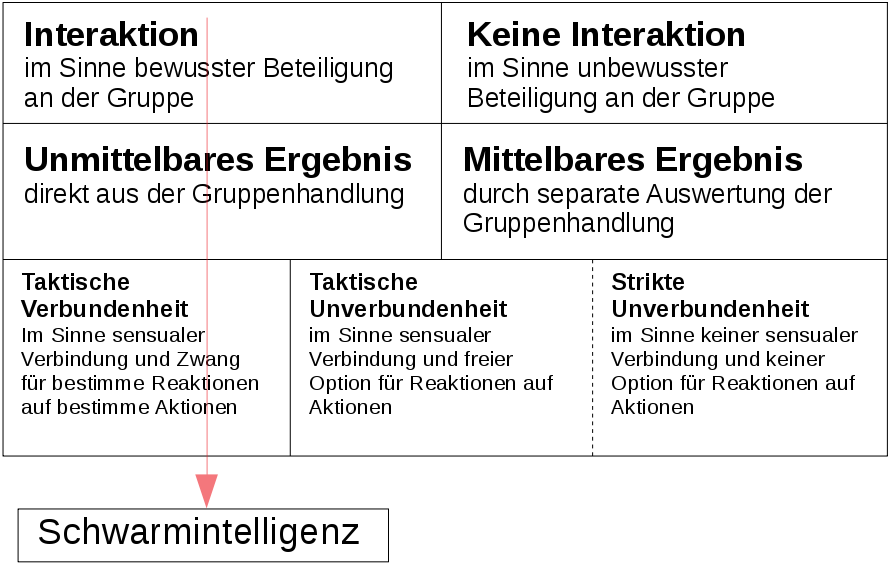
\includegraphics[width=0.8\textwidth]{schwarmintelligenz}
		\label{defabb}
	\end{center}
	\hspace{1in}\parbox{4in}{\caption[Entstehungsbedingung und Definition kollektiver Intelligenz bei Tierschwärmen]{Entstehungsbedingung und Definition kollektiver Intelligenz bei Tierschwärmen\footnotemark}}
\end{figure}
\footnotetext{[1], A. Aulinger (2013)}
\begin{itemize}
	\item \textbf{Interaktion:} Auf Aktion und Reaktion basierende Interaktion gilt als Grundlage für die Definition des Begriffs Schwarmintelligenz. Anlass dafür ist der in den Tieren vorhandene Überlebensinstinkt, der diese veranlasst, sich bewusst an der Gruppe zu beteiligen.
	\item \textbf{Unmittelbares Ergebnis:} Einzelne Tiere führen Handlungen aus ohne Wissen um das Schwarmergebnis. Das Resultat entsteht unmittelbar aus der Handlung des Schwarms und bedarf keiner externen Aggregation und Auswertung.
	\item \textbf{Taktische Verbundenheit:} Sowohl die sensuale Verbindung der Tiere, als auch, der in den Tieren verankerte Instinkt zeugen von der taktischen Verbundenheit des Schwarms bestehend aus festen Aktions- und Reaktionsmustern. 
\end{itemize}
\par Zusammenfassend beschreibt der Begriff Schwarmintelligenz ein Phänomen aus dem Tierreich zur Selbstorganisation eines Schwarms. Damit lebensnotwendige Aufgaben gemeinsam und auf intelligente Weise bewältigen werden. Dabei vollbringen die Tiere im Schwarm Leistungen, die das Vermögen jedes Einzeltiers übersteigen.
\subsubsection{Ameisen}
Ameisen bilden Staaten mit einigen hundert bis zu mehreren Millionen Individuen. Trotz dieser riesigen Anzahl funktioniert ein Ameisenstaat, da er sich selbst organisiert ohne eine hierarchische Instanz, die einen Überblick über alle Aufgaben besitzt oder diese steuert und verteilt. Stattdessen führen die Handlungen einzelner Ameisen im Zusammenspiel zu einem organisierten Staat, der für die Ameisen sorgt und Nahrung, Brutpflege und Schutz bietet. Besonders interessant ist die Fähigkeit effiziente Wege zwischen Futterquelle und Ameisenbau zu finden.\footnote{vgl. [7], L. Pintscher (2008)}.
\par Ist der Futtervorrat des Ameisenbaus erschöpft verlassen mehrere Ameisen den Ameisenbau gleichzeitig und begeben sich auf die Futtersuche. Sobald eine Ameise eine Futterquelle gefunden hat, nimmt sie eine Gewichtseinheit des Futters mit und begibt sich auf den Rückweg zum Ameisenbau. Dabei setzt die Ameise Pheromone frei die mit der Zeit verfliegen, um den Weg zur Futterquelle zu markieren. Die Ameise die den kürzesten Weg zu einer Futterquelle gefunden hat legt die Strecke zwischen Ameisenbau und Futterquelle häufiger zurück.  Die Pheromonspur wird durch das häufige Zurücklegen der Strecke intensiviert und dient als sicherer Wegweiser zur Futterquelle. Mitglieder der Kolonie folgen den intensivsten Pheromonspuren. Ist die Futterquelle erschöpft, löst sich die Pheromonspur auf\footnote{vgl. [11], R. Wehner (2001)}.
\subsubsection{Bienen}
Im kilometerweiten Gelände besitzt keine Biene den gesamten geographischen Überblick. Sie entscheidet nur lokal über die Rentabilität der Futterquelle. Kundschafterinnen und Sammlerinnen, die von der Futtersuche wiederkehren, führen den in Abbildung 2 dargestellten Tanz auf und zeigen unbeschäftigten Bienen damit die Richtung und Entfernung zur gefundenen Futterquelle. Unbeschäftigte Bienen sehen sich die Tänze der im Bienenstock eintreffenden Bienen an und entscheiden sich anschließend für ihr nächstes Ziel. Sobald eine Futterquelle erschöpft ist brauchen die Sammlerinnen länger beim Sammeln und veranlassen aufgrund der geringeren Anzahl an Tänzen weniger Bienen dazu am gleichen Ort zu sammeln\footnote{vgl. [7], L. Pintscher (2008)}.
\begin{figure}[h]
	\begin{center}
		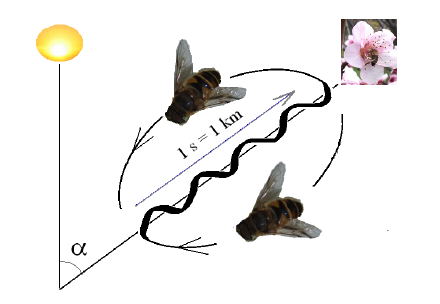
\includegraphics[width=0.5\textwidth]{bienentanz}
		\label{defabb}
	\end{center}
	\hspace{1in}\parbox{4in}{\caption[Der Bienentanz]{Der Bienentanz\footnotemark}}
\end{figure}
\footnotetext{[7], L. Pintscher (2008)}
\newpage
\subsection{Agentenbasierte Modellierung}
Die \ac{ABM} erlaubt eine natürliche Beschreibung von Systemen als eine Sammlung autonomer entscheidungsfähiger Agenten in einer gemeinsamen Umgebung, um emergente Phänomene zu analysieren\footnote{vgl. [2], E. Bonabeau (2002)}. Das Ziel der \acs{ABM} besteht darin, durch die Simulation einer Vielzahl an Agenten, das resultierende Systemverhalten zu untersuchen. Nach C. Macal und M. North\footnote{[6], C. Macal, M. North (2010)} verfügt ein agentenbasiertes Modell über folgende Komponenten:
\begin{itemize}
	\item \textbf{Agenten:} Agenten handeln autonom, proaktiv und reaktionär auf der Basis von festgelegten Regeln. Jeder Agent besitzt nur eine eingeschränkte Sicht auf das Gesamtsystem. Sein Wissen über den globalen Zustand des Systems ist immer unvollständig.
	\item \textbf{Agenten-Beziehungen:} Beziehungen zwischen Agenten entstehen durch die proaktive Aktion eines Agenten und die darauffolgende Reaktion eines anderen Agenten oder Interaktionen der Agenten mit der Umgebung.
	\item \textbf{Agenten-Umgebung:} Agenten interagieren innerhalb einer Umgebung mit anderen Agenten und ihrer Umgebung.
\end{itemize}
\subsubsection{Agenten} 
M. Wooldridge und N. Jennings\footnote{[14], M. Wooldridge, N. Jennings (1995)} weisen Agenten die Charaktereigenschaften Autonomie, Proaktivität, Reaktivität und die Fähigkeit zur Interaktion durch Kommunikation zu. Die Handlungsautonomie eines Agenten beschränkt sich auf die Fähigkeit, eigenständig zu entscheiden, welche der ihm zur Verfügung stehenden Aktionen situationsbedingt auszuführen ist. Zielvorgaben bestimmen wann ein Agent welche Aktionen ausführt. Proaktivität beschreibt dabei das zielgerichtete Verhalten eines Agenten der selbst aktiv wird, statt nur auf die Umgebung zu reagieren.\newline
\subsubsection{Agenten-Beziehungen}
Zwischen den Systemelementen bestehen Interaktionsbeziehungen. Die technischen Voraussetzungen für die Kommunikation werden von der Umgebung bereitgestellt. Beziehungen lassen sich einteilen in Interaktion zwischen Agenten und Umgebung, Interaktion zwischen Agenten und organisatorisch bedingte Beziehungen. Die Kommunikation zwischen Agenten kann dabei direkt durch Austausch von Nachrichten oder indirekt über die Veränderung der Umgebung erfolgen.\newline
\subsubsection{Agenten-Umgebung}
Nach S. Russell und P. Norvig\footnote{[9], S. Russel, P. Norvig (2009)} muss eine geeignete Agenten-Umgebung zugänglich, deterministisch, dynamisch, kontrollierbar und teleologisch sein. Eine zugängliche Umgebung erlaubt den Agenten Zugriff auf ihren Zustand. In der Regel beschränkt sich dieser Zugriff jedoch auf den lokalen Wahrnehmungsbereich eines Agenten und erlaubt somit nur Zugriff auf einen Ausschnitt der Umgebung. Deterministisch ist die Umgebung, sobald der Folgezustand vollständig durch den aktuellen Umgebungszustand und die aktuelle Aktion des Agenten bestimmt ist. Kann sich der Zustand der Umgebung durch Aktionen der Agenten ändern, so handelt es sich um eine dynamische und kontrollierbare Umgebung.
\newpage
\section{Schwarmintelligente Algorithmen}
Die schwarmintelligenten Algorithmen \ac{PSO}, \ac{ACO} und \ac{BCO} orientieren sich an den Strategien der Tierschwärme in der Natur. Die biologische Plausibilität spielt dabei eine untergeordnete Rolle. Im Vordergrund steht die Übertragung der Strategien der Tierschwärme, um Approximationsalgorithmen für Optimierungsprobleme zu entwerfen. Die \acs{PSO} wird in Rahmen dieser Studienarbeit implementiert. Die \acs{ACO} und \acs{BCO} werden vorgestellt um das Verhalten der Tiere und die Übertragung des Verhaltens in Algorithmen besser verstehen zu können.
\subsection{Particle Swarm Optimization}
Die \acs{PSO} wurde erstmals im Jahr 1995 von J. Kennedy und R. Ebert\footnote{[4], J. Kennedy, R. Ebert (1995)} beschrieben. Sie stellt ein, auf der Abfolge von abstrakten Schritten basiertes, Verfahren zur näherungsweisen Lösung von Optimierungsproblemen dar. Zur Lösung des Optimierungsproblems wird eine Population von Partikeln, so lange durch einen Suchraum bewegt, bis eine hinreichende Lösung in einer endlichen Zeit gefunden wird. Dabei stellt die Position eines Partikels eine potentielle Lösung des Optimierungsproblems dar und wird in jedem Zeitschritt neu berechnet\footnote{vgl. [5], Y. Liu (2014)}.
\subsubsection{Suchraum}
Der Suchraum $S \subset \mathbb{R}^n$ ist ein n-dimensionaler Raum, in dem sich die gesamte Population $X=\{x_{1},x_{2},...,x_{n}\}$ der Partikel bewegt. Damit eine Lösung gefunden werden kann beschränkt sich der Suchraum auf eine endliche Anzahl an möglichen Positionen, die von den Partikeln besucht werden können.
\subsubsection{Partikel}
Jeder Partikel $x_{i}$ besitzt folgende Eigenschaften im Suchraum $S$ zum Zeitpunkt $t$:
\begin{itemize}
	\item \textbf{Position $x_{i}(t)$ im Suchraum $S$ mit einem Funktionswert $f(x_{i}(t))$:} Die aktuelle Position des Partikels $x_{i}$ zum Zeitpunkt $t$ repräsentiert eine potentielle Lösung des Optimierungsproblems. Der dazugehörende Funktionswert $f(x_{i}(t))$ beschreibt die Güte der potentiellen Lösung.
	\item \textbf{Position $x_{b,i}(t)$ im Suchraum $S$ mit einem Funktionswert $f(x_{b,i}(t))$:} Die Position $x_{b,i}$ ist die bisher beste Position des Partikels $x_{i}$ zum Zeitpunkt $t$.
	\item \textbf{Position $x_{g}(t)$ im Suchraum $S$ mit einem Funktionswert $f(x_{g}(t))$:} Die Position $x_{g}$ ist die bisher beste Position des Partikelschwarms zum Zeitpunkt $t$.
	\item \textbf{Geschwindigkeit $v_{i}(t)$:} Die Geschwindkeit $v_{i}$ mit der sich der Partikel durch den Suchraum $S$ zum Zeitpunkt $t$ bewegt.
	\item \textbf{Trägheitskoeffizient $w$:} Der Trägheitskoeffizient $w$ bestimmt die Gewichtung der Geschwindigkeit $v_{i}(t)$ zum Zeitpunkt $t+1$.
	\item \textbf{lokaler Vertrauenskoeffizient $a_{l}$:} Der lokale Vertrauenskoeffizient $a_{l}$ bestimmt die Gewichtung der lokalen Attraktion, bei der Berechnung der Geschwindigkeit $v_{i}(t+1)$.
	\item \textbf{globaler Vertrauenskoeffizient $a_{g}$:} Der globale Vertrauenskoeffizient $a_{g}$ bestimmt die Gewichtung der globalen Attraktion, bei der Berechnung der Geschwindigkeit $v_{i}(t+1)$.
\end{itemize}
Der Trägheitskoeffizient $w$ und die Vertrauenskoeffizienten $a_{l}$ und $a_{g}$ geben an, wie sehr die Partikel sich selbst, ihren eigenen Erfahrungen und den Erfahrungen ihrer Nachbarn vertrauen.
\newpage
\subsubsection{Algorithmus}
\begin{framed}
	\begin{algorithm}[H]
		Initialisiere Partikelschwarm $X$ im Suchraum $S$\;
		\While{Maximale Iterationen nicht erreicht}{
			Bestimme für jeden Partikel Position $x_{i}(t)$\;
			Bestimme für jeden Partikel Geschwindigkeit $v_{i}(t)$\;
			Berechne für jeden Partikel den Funktionswert $f(x_{i}(t))$\;
			\lIf{$f(x_{i}(t))$ besser als $f(x_{b,i}(t))$)}{
				Setze $x_{b,i}(t)$ = $x_{i}(t)$
			}
			\lIf{$f(x_{i}(t))$ besser als $f(x_{g}(t))$}{
				Setze $x_{g}(t))$ = $x_{i}(t)$
			}
			Berechne neue Geschwindigkeit $v_{i}(t+1)$ des Partikels $x_{i}$\;
			Berechne neue Position $x_{i}(t+1)$ des Partikels $x_{i}$\;
		}
		\caption{\acs{PSO} Algorithmus}
		\label{psoalgo}
	\end{algorithm}
\end{framed}
Der abgebildete Algorithmus 1 zeigt den Ablauf der \acs{PSO}. Im ersten Schritt wird die Population $X$ mit zufälligen Positionen $x_{i}$ im Suchraum $S$ initialisiert. Bis die Anzahl an maximalen Iterationen nicht erreicht ist wird für jeden Partikel geprüft ob der Funktionswert $f(x_{i}(t))$ für die Position $x_{i}(t)$ besser ist als der Funktionswert $f(x_{i}(t-1))$ im vorherigen Schritt an der Position $x_{i}(t-1)$. Ist der Funktionswert $f(x_{i}(t))$ für die Position $x-{i}(t)$ des Partikels besser, wird die bisher beste Position des Partikels $x_{b,i}(t)$ zu $x_{i}(t)$. Zudem wird für jeden Partikel $x_{i}$ geprüft, ob der aktuelle Funktionswert $f(x_{i}(t))$ des Partikels besser ist als der globale Funktionswert $f(x_{g}(t))$. Ist dies der Fall so wird die global beste Position $x_{g}(t)$ zu $x_{i}(t)$.  Für die nächste Iteration wird die Geschwindigkeit $v_{i}(t+1)$ und die neue Position $x_{i}(t+1)$ des Partikels nach folgenden Formeln berechnet:
\begin{equation}
v_{i}(t+1) = wv_{i}(t) + a_{l}r_{1}(x_{b,i}(t) - x_{i}(t)) + a_{g}r_{2}(x_{g}(t) - x_{i}(t))
\end{equation} 
\begin{equation}
x_{i}(t+1) = x_{i}(t) + v_{i}(t+1)
\end{equation}
\par Bei der Berechnung der neuen Geschwindigkeit $v_{i}(t+1)$ wird die Entfernung der Position  $x_{g}(t)$ zur Position $x_{b,i}(t)$ berechnet. Dabei fallen die Zufallszahlen $r_{1}$, $r_{2} \subset \mathbb{R}$ ins Gewicht, sowie die Parameter $w$, $a_{l}$, $a_{g}$, mit denen das Verhalten des Schwarms verändert wird. Gilt $a_{l} > a_{g}$, dann streben die Partikel in Richtung von $x_{b,i}(t)$. Ist $a_{g} > a_{l}$, dann konvergieren die Partikel zur Position $x_{g}(t)$. Abbildung 2 zeigt in grafischer Darstellung die Berechnung der neuen Geschwindigkeit $v_{i}(t+1)$ und der neuen Position $x_{i}(t+1)$.\newline
\begin{figure}[h]
	\begin{center}
		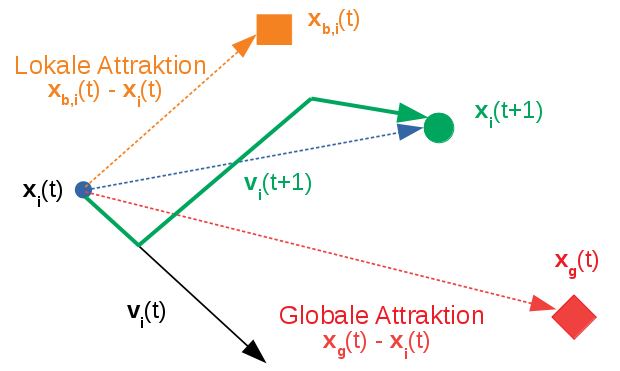
\includegraphics[width=0.58\textwidth]{pso}
	\end{center}
	\hspace{1in}\parbox{4in}{\caption[\acs{PSO}, Berechnung von $x_{i}(t+1)$ und $v_{i}(t+1)$]{Berechnung von $x_{i}(t+1)$ und $v_{i}(t+1)$}}
	\label{psoabb}
\end{figure}
\newpage
\subsection{Ant Colony Optimization}
Die von M. Dorigo vorgestellte \acs{ACO} dient, wie die \acs{PSO}, zur Lösung von Optimierungsproblemen. Zur näherungsweisen Lösung des Optimierungsproblems wird bei der \acs{ACO} eine Population an modellierten Ameisen instanziiert und durch den, vom Optimierungsproblem definierten, Suchraum bewegt. Die Positionen der modellierten Ameisen repräsentieren potentielle Lösungen des Optimierungsproblems und werden in jedem Zeitschritt neu berechnet. Zudem ist jede Position im Suchraum mit einem Pheromonniveau markiert\footnote{vgl. [3], M. Dorigo, M. Birattari, T. Stützle (2004)}.
\subsubsection{Suchraum}
Der Suchraum $S \subset \mathbb{R}^n$ ist ein n-dimensionaler Raum, in dem sich die gesamte Population $X=\{x_{1},x_{2},...,x_{n}\}$ der modellierten Ameisen bewegt. Damit eine Lösung gefunden werden kann beschränkt sich der Suchraum auf eine endliche Anzahl an möglichen Positionen $P=\{p_{1},p_{2},....,p_{n}\}$ die von den modellierten Ameisen besucht werden können. Jeder Position $P$ im Suchraum $S$ ist ein Wert $\tau_{i}$ zugeordnet, der das Pheromonniveau der jeweiligen Position beschreibt.
\subsubsection{Modellierte Ameise}
Jede modellierte Ameise besitzt folgende Eigenschaften im Suchraum $S$ zum Zeitpunkt $t$:
\begin{itemize}
	\item \textbf{Position $x_{i}(t)$ im Suchraum $S$ mit einem Funktionswert $f(x_{i}(t))$:} Die aktuelle Position der modellierten Ameise $x_{i}$ zum Zeitpunkt $t$ repräsentiert eine potentielle Lösung des Optimierungsproblems. Der dazugehörende Funktionswert $f(x_{i}(t))$ beschreibt die Güte der potentiellen Lösung.
	\item \textbf{Position $x_{g}(t)$ im Suchraum $S$ mit einem Funktionswert $f(x_{g}(t))$:} Die Position $x_{g}$ ist die bisher beste Position der Ameisenkolonie zum Zeitpunkt $t$.
	\item \textbf{Teillösungen $C=\{c_{1}(t),c_{2}(t),...,c_{n}(t)\}$ die der modellierten Ameise $x_{i}$ zum Zeitpunkt $t$ zur Verfügung stehen:} Die modellierte Ameise $x_{i}$ wählt aus der ihr zur Verfügung stehenden Teillösungen $C$ zum Zeitpunkt $t$ eine Teillösung. Die gewählte Teillösung entspricht der nächsten Position der modellierten Ameise $x_{i}$ zum Zeitpunkt $t+1$.
	\item \textbf{Wahrscheinlichkeiten $W=\{w_{c_{1}}(t),w_{c_{2}}(t),...,w_{c_{n}}(t)\}$  zur Wahl von $x_{i}(t+1)$:} Die Wahrscheinlichkeiten $W$ werden für die, der modellierten Ameise zur Verfügung stehenden, Teillösungen $C$ berechnet. Die Teillösung mit der höchsten Wahrscheinlichkeit wird von der modellierten Ameise ausgewählt.  	
	\item \textbf{Parameter $\alpha$:} Der Parameter $\alpha$ bestimmt die Gewichtung der Pheromonmarkierungen der Teillösungen $C$ bei der Berechnung der Wahrscheinlichkeiten $W$.
	\item \textbf{Parameter $\beta$:} Der Parameter $\beta$ bestimmt die Gewichtung der Güte der Teillösungen $C$ bei der Berechnung der Wahrscheinlichkeiten $W$
\end{itemize}
Mit $\alpha = 0$ und $\beta = 1$ erhält man einen Greedy-Algorithmus. Umgekehrt erhält man mit $\alpha = 1$ und $\beta = 0$ einen rein zufallsgesteuerten Algorithmus.
\newpage
\subsubsection{Algorithmus}
\begin{framed}
	\begin{algorithm}[H]
		Initialisiere Ameisenkolonie $X$ im Suchraum $S$\;
		\While{Maximale Iterationen nicht erreicht}{
			Berechne für jede modellierte Ameise $x_{i}$ die Wahrscheinlichkeiten $W$ für die möglichen Teillösungen $C$ ausgehend von Position $x_{i}(t)$\;
			Bestimme für jede modellierte Ameise neue Position $x_{i}(t+1)$\;
			\lIf{$f(x_{i}(t+1))$ besser als $f(x_{g}(t))$}{
				Setze $x_{g}(t))$ = $x_{i}(t+1)$
			}
			Berechne für jede gewählte Teillösung die neue Pheromonmarkierung $\tau_{i}(t+1)$ für Position $P$ im Suchraum $S$\;
		}
		\caption{\acs{ACO} Algorithmus}
		\label{acoalgo}
	\end{algorithm}
\end{framed}
Im ersten Schritt des abgebildeten Algorithmus 2 wird die Population $X$ an einer bestimmten Position $P$ im Suchraum $S$ initialisiert. Solange die Anzahl an maximalen Iterationen nicht erreicht ist berechnet jede Ameise die Wahrscheinlichkeiten $W$ für die ihr zur Verfügung stehenden Teillösungen $C$ mit der Formel:
\begin{equation}
W(c_{i}|x_{i}(t)) = \frac{\tau_{c_{i}}^\alpha(t) \cdot [f(c_{i}(t))]^\beta}{\sum_{} c \in C\; \tau_{c}(t)^\alpha \cdot [f(c(t))]^\beta}
\end{equation}
\par Die Wahrscheinlichkeit ist abhängig von dem Pheromonniveau $tau_{c_{i}}$ der jeweiligen Teillösung und der Güte der Teillösung, bestimmt durch $f(c_{i}(t))$. Die Parameter $\alpha$ und $\beta$ verändern das Verhalten der modellierten Ameisen. Gilt $\alpha > \beta$ dann ist das Pheromonniveau der Teillösung ausschlaggebender als die Güte der Teillösung für die Berechnung der Wahrscheinlichkeiten $W$. Sind die Wahrscheinlichkeiten $W$ für alle Teillösungen $C$ berechnet, entscheidet sich die modellierte Ameise für die Teillösung mit der höchsten Wahrscheinlichkeit. Die von der modellierten Ameise gewählte Teillösung entspricht der neuen Position $x_{i}(t+1)$. Im Anschluss wird für jede modellierte Ameise $x_{i}(t)$ geprüft, ob der aktuelle Funktionswert $f(x_{i}(t))$  besser ist als der globale Funktionswert $f(x_{g}(t))$. Ist dies der Fall so wird die global beste Position $x_{g}(t)$ zu $x_{i}(t)$. Am Ende der Iteration werden die Pheromonmarkierungen mit folgender Formel aktualisiert:
\begin{equation}
\tau_{i}(t+1) = (1 - \rho) \tau_{i}(t) + \sum_{x_{i} \in X}\ \Delta \tau_{i}(t)^C
\end{equation}
\par Hierbei ist $\rho$ der konstante Verdunstungsfaktor der Pheromonmarkierungen. Die an der gewählten Teillösung hinterlassene Pheromonmenge $\Delta \tau_{i}(t)^C$ berechnet sich durch die Formel:
\begin{equation}
\Delta \tau_{i}(t)^C = f(c_{i}(t))
\end{equation}
\newpage
\subsection{Bee Colony Optimization}
Die im Zeitraum 1999 bis 2003 von D. Teodorovi\'{c} und P. Lu\u{c}i\'{c}\footnote{[10], D. Teodorovi\'{c}, P. Lu\u{c}i\'{c} (2001)} entwickelte \acs{BCO} stellt, wie die \acs{PSO} und \acs{ACO}, ein metaheuristisches Verfahren zur Lösung von Optimierungsproblemen dar. Die zur näherungsweisen Lösung des Optimierungsproblems, durch den Suchraum bewegten modellierten Bienen repräsentieren potentielle Lösungen des Optimierungsproblems, über ihre Position im Suchraum. 
\subsubsection{Suchraum}
Der Suchraum $S$ der \acs{BCO} unterscheidet sich nicht von dem in Kapitel 3.1.1 beschriebenen Suchraum der \acs{PSO}. 
\subsubsection{Modellierte Biene}
Jede modellierte Biene besitzt folgende Eigenschaften im Suchraum $S$ zum Zeitpunkt $t$:
\begin{itemize}
	\item \textbf{Position $x_{i}(t)$ im Suchraum $S$ mit einem Funktionswert $f(x_{i}(t))$:} Die aktuelle Position der modellierten Biene $x_{i}$ zum Zeitpunkt $t$ repräsentiert eine potentielle Lösung des Optimierungsproblems. Der dazugehörende Funktionswert $f(x_{i}(t))$ beschreibt die Güte der potentiellen Lösung.
	\item \textbf{Position $x_{g}(t)$ im Suchraum $S$ mit einem Funktionswert $f(x_{g}(t))$:} Die Position $x_{g}$ ist die bisher beste Position der Bienenkolonie zum Zeitpunkt $t$.
	\item \textbf{Loyalitätswahrscheinlichkeit $l_{i}(t)$:} Die Loyalitätswahrscheinlichkeit $l_{i}(t)$ der modellierten Biene $x_{i}$ bestimmt den Status $Z$ zum Zeitpunkt $t$.
	\item \textbf{Status $Z$:} Ist die Loyalitätswahrscheinlichkeit $l_{i}(t)$ größer als eine Zufallszahl so wird die modellierte Biene $x_{i}$ zum Zeitpunkt $t$ in den Status Loyal versetzt. Die modellierte Biene erhält den Status Frei sobald die Loyalitätswahrscheinlichkeit kleiner ist als die Zufallszahl.
	\item \textbf{(optional) Rekrutierungsbienen  $R=\{r_{1}(t),r_{2}(t),...,r_{n}(t)\}$ die der modellierten Biene $x_{i}$ zum Zeitpunkt $t$ zur Verfügung stehen:} Die modellierte Biene $x_{i}$ wählt aus der ihr zur Verfügung stehenden Rekrutierungsbienen $R$ zum Zeitpunkt $t$ eine Rekrutierungsbiene. 
	\item \textbf{(optional) Richtung $v_{i}(t)$:} Die Richtung $v_{i}(t)$ von der aktuellen Position $x_{i}(t)$ der modellierten Biene zur gewählten Rekrutierungsbiene $r_{i}(t)$.
\end{itemize}
Befindet sich eine modellierte Biene $x_{i}$ im Status Loyal besitzt sie zum Zeitpunkt $t$ keine Rekrutierungsbienen $R$ sondern ist ihrer Lösung $x_{i}(t)$ gegenüber loyal und wird diese nicht verändern. Ebenso besitzt sie daher keine Richtung $v_{i}(t)$.
\newpage
\subsubsection{Algorithmus}
\begin{framed}
	\begin{algorithm}[H]
		Initialisiere Bienenkolonie $X$ im Suchraum $S$\;
		\While{Maximale Iterationen nicht erreicht}{
			Bestimme für jede modellierte Biene Position $x_{i}(t)$ und berechne den Funktionswert $f(x_{i}(t))$\;
			Bestimme $n$ Rekrutierungsbienen $R$ mit den besten Funktionswerten $f(x_{i}(t))$\;
			Berechne für jede modellierte Biene die Loyalitätswahrscheinlichkeit $l_{i}(t)$\;
				\eIf{$l_{i}(t)$ größer als Zufallszahl}{
					Versetze Biene in den Status Loyal;
				}
				{
					Versetze Biene in den Status Frei;
				}
				\eIf{Biene im Zustand Frei}{
					Berechne Rekrutierungswahrscheinlichkeiten $W$ für Rekrutierungsbienen $R$ und wähle Rekrutierungsbiene $r_{i}(t)$\;
					Bestimme Richtung $v_{i}(t)$ von Position $x_{i}(t)$ zu $r_{i}(t)$\;
					Bewege dich in Richtung $v_{i}(t)$\;
				}
				{
					Setze neue Position $x_{i}(t+1)$ = $x_{i}(t)$\;
				}	
				\lIf{$f(x_{i}(t+1))$ besser als $f(x_{g}(t))$}{
					Setze $x_{g}(t))$ = $x_{i}(t+1)$
				}		
		}
		\caption{\acs{BCO} Algorithmus}
		\label{bcoalgo}
	\end{algorithm}
\end{framed}
Der erste Schritt des abgebildeten Algorithmus 3 ist die Initialisierung der modellierten Bienen im Suchraum $S$. Bis die maximale Anzahl an Iterationen nicht erreicht ist wird in jeder Iteration die aktuelle Position der modellierten Biene und der dazugehörige Funktionswert $f(x_{i}(t))$ der potentiellen Lösung bestimmt. Im Anschluss werden $n$ modellierte Bienen mit den besten Funktionswerten ausgewählt. Diese Bienen stellen die Rekrutierungsbienen $R$ dar. Für jede modellierte Biene, ausgenommen die Rekrutierungsbienen, wird im nächsten Schritt die Loyalitätswahrscheinlichkeit $l_{i}(t)$ nach folgender Formel berechnet:
\begin{equation}
l_{i}(t) = e^{-\frac{f(x_{g}(t))-f(x_{i}(t))}{Anzahl der Iterationen}}
\end{equation}
\par Die modellierten Bienen werden nach der Berechnung der Loyalitätswahrscheinlichkeit $l_{i}(t)$ in den Status Loyal oder Frei versetzt. Befindet sich eine modellierte Biene im Status Loyal hält sie an ihrer Lösung $x_{i}(t)$ fest. Wird die modellierte Biene in den Status Frei versetzt werden die Rekrutierungswahrscheinlichkeiten zur Wahl der Rekrutierungsbienen nach folgender Formel berechnet:
\begin{equation}
r_{i}(t) = \frac{f(r_{i}(t)}{\sum_{r \in R}\ f(r(t))}
\end{equation}
\par Jede modellierte Biene im Status Frei wählt anschließend eine Rekrutierungsbiene $r_{i}(t)$ auf der Grundlage der berechneten Rekrutierungswahrscheinlichkeiten. Im Anschluss wird die Richtung $v_{i}(t)$ von der Position modellierten Biene $x_{i}(t)$ zu der gewählten Rekrutierungsbiene $r_{i}(t)$ bestimmt. Im letzten Schritt der Iteration bewegt sich die modellierte Biene auf die Lösung ihrer Rekrutierungsbiene zu.
\newpage
\section{Modelle und Frameworks}
\subsection{Modelle}
Als abstraktes Beispiel wird die \acs{PSO} angeführt. Die \acs{PSO} wird in dieser Arbeit dazu verwendet das globale Minimum der Rastrigin-Funktion zu finden. Bei der Modellierung der Futtersuche von Ameisen und Bienen sollen die Strategien der Tiere, zum effizienten Abbau einer Futterquelle, berücksichtigt werden. Das Modell der Futtersuche von Ameisen und Bienen soll keine Implementierung der vorgestellten schwarmintelligenten Algorithmen \acs{ACO} und \acs{BCO} darstellen, sondern eine möglichst realitätsnahe Simulation der Futtersuche der Tiere in der Natur zulassen. 
\subsubsection{Finden des globalen Minimums einer Funktion mit der \acs{PSO}}
\paragraph{Modellbeschreibung}
Im Modell werden Partikel durch die zweidimensionale Agenten - Umgebung bewegt, um das globale Minimum der, in Abbildung 3 abgebildeten, zweidimensionalen Rastrigin-Funktion zu finden. Die Rastrigin-Funktion wurde 1974 von A. Leonard vorgeschlagen und dient der Performanceanalyse von Optimierungsalgorithmen\footnote{[13], Wikipedia (2016)}. Die Rastrigin-Funktion ist definiert durch:\newline
\begin{equation}
f(x) = An +  \sum_{i=0}^n \ [x_{i}^2 - A \cos (2\pi x_{i})]
\end{equation}
Dabei ist $A = 10$ eine Konstante, $n$ die Dimensionen. Außerdem gilt $x = {x_{1},...,x_{n}}$ mit $x_{i} \in [-5.12,5.12]$.\newline
\begin{figure}[h]
	\begin{center}
		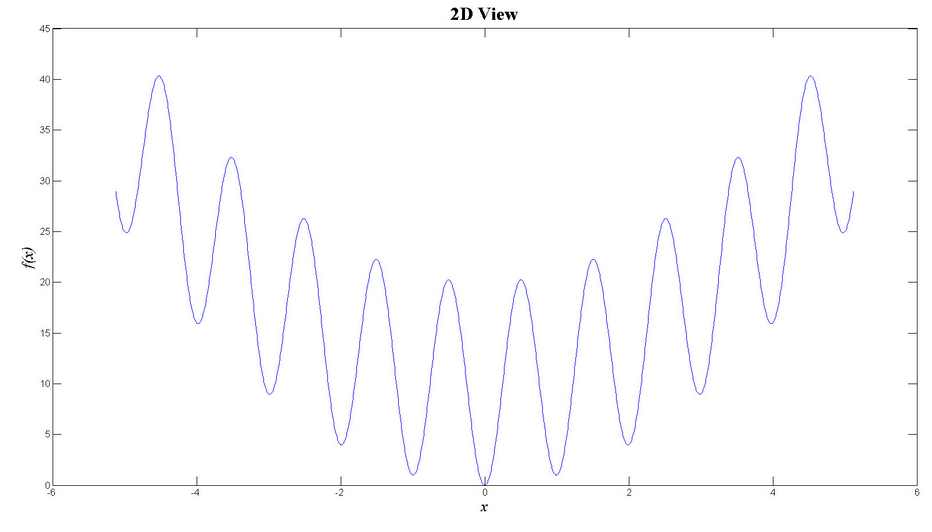
\includegraphics[width=1\textwidth]{rastrigin}
	\end{center}
	\hspace{1in}\parbox{4in}{\caption[zweidimensionale Rastrigin-Funktion]{Zweidimensionale Rastrigin-Funktion\footnotemark}}
	\label{rastabb}
\end{figure}
\footnotetext{Bildquelle: http://al-roomi.org/benchmarks/unconstrained/n-dimensions/174-generalized-rastrigin-s-function}
\paragraph{Methode}
Das Modell zur Simulation der \acs{PSO} ist in dieser Arbeit als abstraktes Beispiel für agentenbasierten Modellierung angeführt. Die Methode zum Finden des globalen Minimums der Rastrigin-Funktion stellt der im Kapitel 3.3 vorgestellte \acs{PSO}-Algorithmus dar.
\paragraph{Parameter}
Im Modell ist die Anzahl der Partikel, der lokale Vertrauenskoeffizient und der globale Vertrauenskoeffizient einstellbar.
\subsubsection{Die Futtersuche von Ameisen und Bienen}
\paragraph{Modellbeschreibung}
Im Modell der Futtersuche suchen die Agenten nach einer Futterquelle in einer zweidimensionalen Agenten-Umgebung. Sie starten ihre Suche im Ameisenbau oder Bienenstock. Das erste Ziel des Modells ist das zufallsgesteuerte Finden der Futterquelle durch die Agenten. Im Anschluss interagieren die Agenten miteinander um die Futterquelle möglichst effizient abzubauen. Um die Effizienz der Methoden in Experimenten zu messen wird die Anzahl der gesammelten Futtereinheiten in einem bestimmten Zeitraum ermittelt. 
\paragraph{Methode der Ameisen}
Zum effizienten Abbau der Futterquelle kommunizieren die modellierten Ameisen über die zweidimensionale Agenten-Umgebung in Form von Pheromonmarkierungen. Im Modell gibt es zwei Pheromontypen, die mit der Zeit verdunsten. Heimatpheromone markieren den Weg zum Ameisenbau und Futterpheromone den Weg zur Futterquelle. Auf der Suche nach der Futterquelle werden Heimatpheromone hinterlassen. Findet eine modellierte Ameise die Futterquelle wird eine Einheit der Futterquelle abgebaut. Nachdem die Futterquelle abgebaut wurde kehrt die Ameise zum Ameisenbau zurück. Dabei hinterlässt sie Futterpheromone. Befindet sich die modellierte Ameise im Ameisenbau liefert sie die Futtereinheit ab und begibt sich anschließend erneut auf Futtersuche. Der abgebildete Algorithmus \ref{futtersucheaco} fasst das Vorgehen für den Abbau der Futterquelle zusammen.
\begin{framed}
	\begin{algorithm}[H]
			\eIf{hatFuttereinheit}
			{
				Kehre zum Ameisenbau zurück (Folge Heimatpheromonen)\;
				Hinterlasse Futterpheromone\;
				\lIf{Position der Ameise == Position des Ameisenbaus}{
					hatFuttereinheit = false
				}
			}
			{
				Finde Futterquelle (Folge Futterpheromonen)\;
				Hinterlasse Heimatpheromone\;
				\lIf{Position der Ameise == Position der Futterquelle}{
					hatFuttereinheit = true
				}
			}
		\caption{Futtersuche Ameisen}
		\label{futtersucheaco}
	\end{algorithm}
\end{framed}
\paragraph{Parameter Ameisen}
Die einstellbaren Parameter des Modells sind die Anzahl der modellierten Ameisen und die Wahrscheinlichkeiten mit denen sich die Ameisen an die Pheromonmarkierungen folgen oder zufällig handeln in Form der Parameter $\alpha$ und $\beta$.
\paragraph{Methode der Bienen}
Um die Futterquelle möglichst effizient abzubauen kommunizieren die modellierten Bienen über den  Bienentanz. Findet eine modellierte Biene die Futterquelle kehrt sie zum Bienenstock zurück. Dort tanzt sie für andere Bienen um ihnen die Richtung und Entfernung der Futterquelle mitzuteilen. Bienen die den Tanz beobachtet haben verlassen den Bienenstock und fliegen an die ihnen mitgeteilte Position. Um die exakte Position der Futterquelle ausfindig zu machen, suchen die modellierten Bienen im Umkreis der ihnen durch den Tanz mitgeteilten Position. Finden die modellierten Bienen die Futterquelle kehren sie zum Bienenstock zurück und tanzen, um weiteren Bienen die Position der Futterquelle mitzuteilen. Der abgebildete Algorithmus 5 fasst das Vorgehen der Bienen zusammen.
\begin{framed}
	\begin{algorithm}[H]
		\eIf{InformationFutterquelle}
		{
			Bewege dich in die Richtung der Futterquelle\;
			Finde die Futterquelle\;
			Kehre zum Bienenstock zurück\;
			Tanze\;
		}
		{
			\eIf{Tanzende Biene in der Umgebung}{
				Beobachte tanzende Biene\;
				InformationFutterquelle = true\;
			}
			{
				Starte zufällige Suche nach der Futterquelle\;
				\eIf{Suchlimit}{
					Kehre zum Bienenstock zurück\;
				}
				{
					Finde die Futterquelle\;
					InformationFutterquelle = true\;
					Kehre zum Bienenstock zurück\;
					Tanze\;					
				}	
			}
		}
		\caption{Futtersuche Bienen}
		\label{futtersuchebco}
	\end{algorithm}
\end{framed}
\paragraph{Parameter Bienen}
Im Modell ist die Anzahl der modellierten Bienen einstellbar.
\subsection{Framework}
Zur Implementierung der in Kapitel 4.1 definierten Modelle wird ein Framework verwendet. Für die \acs{ABM} stehen mehrere Softwareplattformen und Bibliotheken zur Verfügung. Zu den bekanntesten und meistgenutzten Plattformen gehören NetLogo, MASON, Swarm und Repast.
\subsubsection{Anforderungen}
Die Anforderungen an das Framework zur Erstellung der in Kapitel 4.1 vorgestellten Modelle und anschließender grafischer Simulation sind:
\begin{itemize}
	\item \textbf{Open-Source + kostenlos:} Der Quelltext des Frameworks ist öffentlich. Zudem kann das Framework kostenlos genutzt werden.
	\item \textbf{Aktualität:} Es ist eine aktuelle und stabile Version des Frameworks verfügbar. 
	\item \textbf{Einsetzbarkeit:} Das Framework kann auf dem Betriebssystem Linux verwendet werden und unterstützt die Programmiersprache Java. Diese Anforderung entsteht durch die Präferenzen des Autors dieser Arbeit.
	\item \textbf{Visualisierung:} Modelle werden grafisch in 2D simuliert.
	\item \textbf{Dokumentation + Tutorial:} Das Framework ist umfangreich dokumentiert und besitzt ein Tutorial für Einsteiger.
	\item \textbf{Ausführungsgeschwindigkeit der Simulation:} Die Ausführungsgeschwindigkeit der Simulation ist hoch, trotz rechenintensiven Modellen mit vielen Agenten und Iterationen.
\end{itemize}
\subsubsection{Übersicht}
\paragraph{NetLogo}
NetLogo ist eine Open-Source-Plattform und wurde 1999 von U. Wilensky entwickelt. Die neuste Version 6.0.3 wurde im März 2018 veröffentlicht und steht für die Betriebssysteme Mac, Windows und Linux zur Verfügung. Die proprietäre funktionale Programmiersprache und die ausführliche Dokumentation machen es Einsteigern ohne Programmierkenntnisse einfach erste eigene Modelle zu implementieren. Das Fehlen objektorientierter Features schränkt die Funktionalität und Erweiterbarkeit des Frameworks jedoch ein. Darüber hinaus verfügt NetLogo über keine explizite Unterstützung für die Trennung zwischen Agenten, Agenten-Beziehungen und Agenten-Umgebung.
\paragraph{MASON}
\ac{MASON} ist eine Java-Bibliothek, die ein breitgefächertes Repertoire an Funktionen für die \acs{ABM} bereitstellt. Die aktuelle Version 1.9 wurde im Juni 2015 veröffentlicht. Eine umfangreiche Dokumentation der Open-Source-Bibliothek und ein einsteigerfreundliches Tutorial erlauben es innerhalb weniger Stunden eine erste lauffähige Simulation zu erstellen.
\paragraph{Swarm}
Swarm ist eine der ersten \acs{ABM}-Plattformen. Ursprünglich wurde Swarm 1997 am Santa Fe Institute entwickelt und veröffentlicht. Die ABM-Plattform Swarm war zuerst nur auf UNIX-basierten Betriebssystemen einsetzbar und unterstützte nur die Programmiersprache Objective-C. Heute steht Swarm für die Betriebssysteme Mac, Windows und Linux zur Verfügung und unterstützt neben Objective-C auch Java. Das Framework ist Open-Source. Version 2.4.1 wurde im April 2009 veröffentlicht.
\paragraph{Repast}
Repast ist eine Open-Source-Plattform für die \acs{ABM}. Die Software ist für die Betriebssysteme Mac, Windows und Linux verfügbar. Es existieren zwei verschiedene Editionen der Plattform. Repast Simphony implementiert grundlegende und erweiterte Konzepte der \acs{ABM}. Unterstützt werden die Programmiersprachen Java, Logo und Groovy. Repast High Performance Computing ist ein agentenbasiertes Modellierungssystem speziell entwickelt für die parallele Ausführung der Simulationen auf verteilten Systemen. Zur Modellentwicklung mit dieser Edition von Repast werden umfangreiche Programmierkenntnisse in C++ vorausgesetzt. Die stabile Version 2.5 von Repast Symphonie wurde im Oktober 2017 veröffentlicht. 
\paragraph{Zusammenfassung}
S. Railsback, S. Lytinen und S. Jackson\footnote{vgl. [8], S. Railsback, S. Lytinen, S. Jackson (2006)} untersuchten verschiedene Plattformen für die \acs{ABM} und Simulation. Ihre Ergebnisse über die oben genannten \acs{ABM}-Plattformen können folgendermaßen zusammengefasst werden:
\begin{itemize}
	\item \textbf{NetLogo:} Netlogo ist einfach zu bedienen und besitzt eine umfangreiche Dokumentation. NetLogo ist eine gute Wahl für simple Modelle bei denen die Ausführungszeit der Simulation eine untergeordnete Rolle spielt. Außerdem eignet sich NetLogo zur Erstellung eines Modellprototyps. Dieser Prototyp kann anschließend in anderen \acs{ABM}-Plattformen erweitert werden.
	\item \textbf{MASON:} MASON ist eine gute Wahl für erfahrene Programmierer, die an rechenintensiven Modellen mit vielen Agenten und Iterationen arbeiten. Ein Vorteil von MASON ist die Reproduzierbarkeit der Simulationsergebnisse auf verschiedenen Betriebssystemen.
	\item \textbf{Swarm:} Swarm ist stabil, klein, gut organisiert und unterstützt komplexe Modelle. Voraussetzung für einen schnellen Einstieg ist Programmiererfahrung mit Objective-C.
	\item \textbf{Repast:} Repast ist die vollständigste \acs{ABM}-Plattform und hat eine vergleichsweise schnelle Ausführungszeit der Simulationen. Die Dokumentation ist teilweise unvollständig.
\end{itemize}
\subsubsection{Auswahl}
Tabelle \ref{tabframework1} zeigt eine Übersicht der Frameworks und die erfüllten Anforderungen.
Zur Implementierung der in Kapitel 4.1 beschriebenen Modelle wird MASON als Framework gewählt. Mit MASON können die Modelle in Java implementiert werden. Da im Zuge dieser Studienarbeit rechenintensive Simulationen mit vielen Agenten durchgeführt werden sollen ist die hohe Ausführungsgeschwindigkeit der Simulationen wichtig. MASON bietet zudem eine umfangreiche Dokumentation und ein 14-stufiges Tutorial. 
\begin{table}[h]
	\begin{tabular}{p{1.5cm}|p{1.5cm}|p{1.6cm}|p{1.7cm}|p{1.3cm}|p{1.3cm}|p{2.7cm}}
		& Open-Source + kostenlos & Aktuali-tät & Einsetz-barkeit & Visuali-sierung & Doku + Tutorial & Geschwindig-keit\\ \hline\hline
		NetLogo & $\surd$ & Mrz. 2018 & $X$ & 2D/3D & $\surd$ & langsam\\ \hline
		Mason & $\surd$ & Jun. 2015 & $\surd$ & 2D/3D & $\surd$ & sehr schnell\\ \hline
		Swarm & $\surd$  & Apr. 2009 & $\surd$ & 2D/3D & $X$ & langsam\\ \hline
		Repast & $\surd$ & Okt. 2017 & $\surd$ & 2D/3D & $\surd$ & schnell\\ \hline
	\end{tabular}
	\caption{Auswahl des Frameworks}
	\label{tabframework1}
\end{table}
\newpage
\section{Implementierung}
Im folgenden Kapitel wird die Implementierung der in Kapitel 4.1 definierten Modelle beschrieben. Auf eine Beschreibung der 2D-Visualisierung für die grafische Simulation der Modelle wird im Umfang dieser Arbeit verzichtet.
\subsection{Finden des globalen Minimums der Rastrigin-Funktion mit der \acs{PSO}}
Die Implementierung des Modells basiert auf der Arbeit von A. Desai und S. Luke. Ihr Modell wurde unter der Academic Free License 3.0 veröffentlich. Das Modell darf modifiziert und anschließend veröffentlicht werden. Um die Implementierung des in Kapitel 4.1.1 definierten Modells zu erläutern wird die Implementierung anhand der Schritte des \acs{PSO}-Algorithmus aus Kapitel 3.1.3 beschrieben.
\subsubsection{Initalisiere Partikelschwarm im Suchraum}
Im ersten Schritt des Modells wird die ausgewählte Anzahl von Partikeln an zufälligen Positionen im Suchraum mit zufälligen Ausgangsgeschwindigkeiten initialisiert. Listing \ref{psomod1} zeigt den Programmcode für die Initialisierung des Partikelschwarms.\newline 
\begin{lstlisting}[caption= PSO: Initalisierte Partikelschwarm im Suchraum,label = psomod1]
public void start(){
	super.start();	
	particles = new Particle[numParticles];
	space = new Continuous2D(height, width);
	//Waehle Rastrigin-Funktion
	Evaluatable f = mapFitnessFunction(fitnessFunction);            
	//Initalisiere Partikel
	for (int i = 0; i < numParticles; i++){
		double x = (random.nextDouble() * width) - (width * 0.5);
		double y = (random.nextDouble() * height) - (height * 0.5);
		double vx = (random.nextDouble() * initialVelocityRange) - (initialVelocityRange * 0.5);
		double vy = (random.nextDouble() * initialVelocityRange) - (initialVelocityRange * 0.5);
		final Particle p = new Particle(x, y, vx, vy, this, f, i);
		particles[i] = p;
	}
}
\end{lstlisting}
\subsubsection{Bestimme Position und Geschwindigkeit}
Nach der Initialisierung wird die Position und Geschwindigkeit der Partikel bestimmt. Listing \ref{psomod2} zeigt den Programmcode zur Bestimmung der Position und Geschwindigkeit.\newline
\begin{lstlisting}[caption= PSO: Bestimme Position und Geschwindigkeit,label = psomod2]
public Particle(double x, double y, double vx, double vy, PSO pso, Evaluatable f) {
	super();
	//Bestimme Position und Geschwindigkeit der Partikel
	this.position.setTo(x, y);
	this.velocity.setTo(vx, vy);
	this.pso = pso;
	this.fitnessFunction = f;
	pso.space.setObjectLocation(this,new Double2D(position));
}
\end{lstlisting}
\subsubsection{Bestimme den Fitnesswert}
Das globale Minimum der Rastrigin-Funktion befindet sich bei den Koordinaten $x=0$ mit $f(x)=0$. Der Fitnesswert bestimmt die Güte der potentiellen Lösung eines Partikels. Von einem gewählten Maximalwert von 1000 wird durch die Berechnung in Listing \ref{psomod3} ein bestimmter Wert abgezogen. Dieser Wert ist abhängig von der Position des Partikels. Je näher die Position des Partikels zum globalen Minimum der Rastrigin-Funktion, desto größer ist der Fitnesswert des Partikels. \newline
\begin{lstlisting}[caption= PSO: Bestimme Fitnesswert,label = psomod3]
public class Rastrigin implements Evaluatable{
	private static final long serialVersionUID = 1;
	//Maximalwert 1000 
	public double calcFitness(double x, double y){
		return (1000 - (20 + x*x - 10*Math.cos(2*Math.PI*x) + y*y - 10*Math.cos(2*Math.PI*y)));
	}
}
\end{lstlisting}
\subsubsection{Bestimme beste Position}
Ist der aktuelle Fitnesswert eines Partikels größer als der in den vorausgehenden Schritten erreichte Fitnesswert des Partikels, dann handelt es sich um die bisher beste Position des Partikels. In jeder Iteration des Modells wird zudem der Partikel mit dem höchsten Fitnesswert bestimmt. Listing \ref{psomod4} prüft, ob die aktuelle Position die bisher beste Position des Partikels ist.\newline
\begin{lstlisting}[caption= PSO: Bestimme beste Position,label = psomod4]
public void updateBest(double currVal, double currX, double currY){
	if (currVal > bestVal){
		bestVal = currVal;
		bestPosition.setTo(currX, currY);
		pso.updateBest(currVal, currX, currY);
	}
}
\end{lstlisting}
\subsubsection{Berechne neue Geschwindigkeit}
Listing \ref{psomod5} zeigt die getrennte Berechnung der x- und y-Komponente der neuen Geschwindigkeit des Partikels. Bei der Berechnung der neuen Geschwindigkeit werden die Vertrauenskoeffizienten berücksichtigt.\newline
\begin{lstlisting}[caption= PSO: Berechne neue Geschwindigkeit,label = psomod5]
public void stepUpdateVelocity(){
	//Berechne x-Komponente
	double inertia = velocity.x;
	double pDelta = bestPosition.x - x;
	double gDelta = pso.bestPosition.x - x;
	double pWeight = pso.localTrust;
	double gWeight = pso.globalTrust;
	//Einfluss der Vertrauenskoeffizienten
	double vx = (0.9*inertia + pWeight*pDelta + gWeight*gDelta) / (1+pWeight+gWeight);
	velocity.setTo(vx, vy);         
}
\end{lstlisting}
\subsubsection{Berechne neue Position}
Listing \ref{psomod6} zeigt den letzten Schritt einer Iteration des Modells. Für die nächste Iteration wird die neue Position des Partikels berechnet. Hierfür wird die in Listing \ref{psomod5} berechnete Geschwindigkeit mit der aktuellen Position des Partikels addiert.\newline
\begin{lstlisting}[caption= PSO: Berechne neue Position,label = psomod6]
public void stepUpdatePosition(){
	position.addIn(velocity);
	pso.space.setObjectLocation(this, new Double2D(position));
}
//Defintion von addIn
public final MutableDouble2D addIn(final MutableDouble2D other){
	x = other.x + x;
	y = other.y + y;
	return this;
}
\end{lstlisting}
\subsection{Die Futtersuche von Ameisen}
Die Implementierung des Modells orientiert sich an der von Arbeit von L. Panait und S. Luke\footnote{http://cs.gmu.edu/~eclab/papers/panait04ant.pdf } und wird anhand der in Kapitel 4.1.2 definierten Methode beschrieben. 
\subsubsection{Kehre zum Ameisenbau zurück}
Hat die modellierte Ameise die Futterquelle gefunden, dann kehrt sie zum Ameisenbau zurück. Dafür prüft der Programmcode in Listing \ref{acomod1} das Heimatpheromonniveau in ihrer Umgebung. Die Entscheidung für welchen Weg sich die modellierte Ameise entscheidet ist abhängig von den Parametern $\alpha$ und $\beta$.\newline
\begin{lstlisting}[caption= Ameisen: Kehre zum Ameisenbau zurück,label = acomod1]
if (hasFoodItem) {
	double max = -1; int max_x = x; int max_y = y;	
	for(int dx = -1; dx < 2; dx++) {
		for(int dy = -1; dy < 2; dy++) {
			int _x = dx+x;
			int _y = dy+y;
			//Pruefe ob sich Position in der Umgebung befindet
			if ((dx == 0 && dy == 0) || _x < 0 || _y < 0 || _x >= AntsForage.GRID_WIDTH || _y >= AntsForage.GRID_HEIGHT) continue;
			//Heimatpheromonkonzentration an der Position(_x,_y)
			double m = af.toHomeGrid.field[_x][_y];
			if (m > max || (m == max) 
			{max = m; max_x = _x; max_y = _y;}
		}
	}
    //Siehe Kapitel 5.3.5 fuer Einfluss des Parameters beta
    //Siehe Kapitel 5.3.6 fuer Einfluss des Parameters alpha
    //Setze neue Position der modellierten Ameise
    af.buggrid.setObjectLocation(this, new Int2D(max_x, max_y));
    //Ameise befindet sich im Ameisenbau
    if (af.sites.field[max_x][max_y] == AntsForage.HOME)
    {hasFoodItem = ! hasFoodItem; }
}
\end{lstlisting}
\subsubsection{Hinterlasse Futterpheromone}
Auf der Rückkehr zum Ameisenbau hinterlässt die modellierte Ameise Futterpheromone, um den Weg zur Futterquelle zu markieren. Dafür wird das Futterpheromonniveau jeder besuchten Position, nach dem in Listing \ref{acomod2} abgebildeten Programmcode, erhöht.\newline
\begin{lstlisting}[caption= Ameisen: Hinterlasse Futterpheromone,label = acomod2]
if (hasFoodItem) { 
	double max = af.toFoodGrid.field[x][y];
	int max_x = x;
	int max_y = y;	
	for(int dx = -1; dx < 2; dx++){
		for(int dy = -1; dy < 2; dy++) {
			int _x = dx+x;
			int _y = dy+y;	
			double m = af.toFoodGrid.field[_x][_y] * (dx * dy != 0 ? af.diagonalCutDown : af.updateCutDown);
			if (m > max) {max = m;}
		}
	}
	//Markiere Position mit Pheromonniveau
	af.toFoodGrid.field[x][y] = max;
}
\end{lstlisting}
\subsubsection{Finde Futterquelle}
Listing \ref{acomod3} zeigt den Programmcode für die Orientierung der modellierten Ameise am Futterpheromonniveau der Positionen in ihrer direkten Umgebung. Der von der modellierten Ameise ausgewählte Weg ist abhängig von den Parametern $\alpha$ und $\beta$.\newline
\begin{lstlisting}[caption= Ameisen: Finde Futterquelle,label = acomod3]
else {
	double max = -1;
	int max_x = x;
	int max_y = y;
	for(int dx = -1; dx < 2; dx++) {
		for(int dy = -1; dy < 2; dy++) {
			int _x = dx+x;
			int _y = dy+y;	
			//Pruefe ob sich Position in der Umgebung befindet		
			if ((dx == 0 && dy == 0) || _x < 0 || _y < 0 || _x >= AntsForage.GRID_WIDTH || _y >= AntsForage.GRID_HEIGHT) continue;
			//Futterpheromonniveau an der Position(_x,_y)
			double m = af.toFoodGrid.field[_x][_y];
			if (m > max || (m == max && state.random.nextBoolean(1.0 / count++))){
				max = m; max_x = _x; max_y = _y;
			}
		}
	}
	//Siehe Kapitel 5.3.5 fuer Einfluss des Parameters beta
	//Siehe Kapitel 5.3.6 fuer Einfluss des Parameters alpha
	//Setze neue Position der modellierten Ameise
	af.buggrid.setObjectLocation(this, new Int2D(max_x, max_y));
	//Ameise befindet sich bei der Futterquelle
	if (af.sites.field[max_x][max_y] == AntsForage.FOOD)
	{hasFoodItem = ! hasFoodItem;}
}
\end{lstlisting}
\subsubsection{Hinterlasse Heimatpheromone}
Auf der Suche nach der Futterquelle hinterlässt die modellierte Ameise Heimatpheromone um den Weg zum Ameisenbau zu markieren. Dafür erhöht sie das Heimatpheromonniveau jeder besuchten Position, durch den in Listing \ref{acomod4} abgebildeten Programmcode. \newline
\begin{lstlisting}[caption= Ameisen: Hinterlasse Heimatpheromone,label = acomod4]
else {
	double max = af.toHomeGrid.field[x][y];
	int max_x = x;
	int max_y = y;
	for(int dx = -1; dx < 2; dx++){
		for(int dy = -1; dy < 2; dy++){
			int _x = dx+x;
			int _y = dy+y;
			double m = af.toHomeGrid.field[_x][_y] * (dx * dy != 0 ? af.diagonalCutDown : af.updateCutDown);
			if (m > max) {max = m;}
		}
	}
	af.toHomeGrid.field[x][y] = max;
}
\end{lstlisting}
\subsubsection{Parameter $\beta$}
Parameter $\beta$ bestimmt mit welcher Wahrscheinlichkeit sich die modellierten Ameisen auf ihrem Weg an die Pheromonmarkierungen halten. \newline
\begin{lstlisting}[caption= Ameisen: Parameter beta,label = acomod5]
if (max == 0 && last != null) {
	if (state.random.nextBoolean(af.paramBeta)){
		int xm = x + (x - last.x);
		int ym = y + (y - last.y);
		if (xm >= 0 && xm < AntsForage.GRID_WIDTH && ym >= 0 && ym < AntsForage.GRID_HEIGHT){ 
			max_x = xm; max_y = ym; 
		}
	}
}
\end{lstlisting}
\subsubsection{Parameter $\alpha$}
Parameter $\alpha$ bestimmt die Wahrscheinlichkeit mit der sich die modellierten Ameisen über die Pheromonmarkierungen hinwegsetzen und zufällig handeln.\newline
\begin{lstlisting}[caption= Ameisen: Parameter alpha,label = acomod6]
else if (state.random.nextBoolean(af.paramAlpha)){
	int xd = (state.random.nextInt(3) - 1); 
	int yd = (state.random.nextInt(3) - 1);
	int xm = x + xd; int ym = y + yd;
	if (!(xd == 0 && yd == 0) && xm >= 0 && xm < AntsForage.GRID_WIDTH && ym >= 0 && ym < AntsForage.GRID_HEIGHT){ 
		max_x = xm;	max_y = ym; 
	}
}
\end{lstlisting}
\subsubsection{Verdunstung der Pheromone}
Zu jeder Iteration des Modells verdunsten die Pheromonmarkierungen auf der Agenten-Umgebung. Dazu wird ein konstanter Verdunstungsfaktor verwendet. Listing \ref{acomod7} zeigt die Programmcode zur Umsetzung der Verdunstung.\newline
\begin{lstlisting}[caption= Ameisen: Verdunstung der Pheromone,label = acomod7]
schedule.scheduleRepeating(Schedule.EPOCH,1, new Steppable(){
	//Verdunstung der Pheromonmarkierungen Verdunstungsfaktor pro Iteration
	public void step(SimState state) { toFoodGrid.multiply(evaporationConstant); toHomeGrid.multiply(evaporationConstant); }}, 1);
}
\end{lstlisting}

\subsection{Die Futtersuche von Bienen}
Die Implementierung des Modells orientiert sich an der Implementierung der Futtersuche von Bienen von Jörg Höhne und wird anhand der in Kapitel 4.1.2 definierten Methode beschrieben.
\subsubsection{Zufällige Suche nach der Futterquelle}
Befindet sich die modellierte Biene im Bienenstock und hat keine Information über die Futterquelle begibt sie sich mit einer niedrigen Wahrscheinlichkeit auf die zufallsgesteuerte Suche nach der Futterquelle. Die Suche ist begrenzt auf eine maximale Anzahl von Suchschritten. Findet die modellierte Biene die Futterquelle innerhalb der maximalen Anzahl an Suchschritten nicht, kehrt sie zum Bienenstock zurück. Listing \ref{bcomod1} zeigt den Programmcode der zufallsgesteuerten Suche nach der Futterquelle.\newline
\begin{lstlisting}[caption= Bienen: Zufällige Suche nach der Futterquelle,label = bcomod1]
protected void doStateInHiveWithoutInfo(){
	//Starte zufaellige Suche nach der Futterquelle mit geringer Wahrscheinlichkeit
	double pStartScouting = getSimulation().pStartScouting;
	if ((pStartScouting) >= r.nextDouble()){
		if (getFoodSource() == null){setState(State.scouting);}
	}
}

protected void doStateScouting(){
	if (r.nextInt(5) == 0) {
		turnBy(Math.toRadians(r.nextInt(40) - 20), Math.toRadians(r.nextInt(40) - 20));
	}
	//Pruefung ob Futterquelle gefunden wurde
	foundSource();
	scoutSteps--;
	if (scoutSteps <= 0){setState(State.returnWithoutInfo);}
}
\end{lstlisting}
\newpage
\subsubsection{Bewegung in Richtung der Futterquelle}
Besitzt die modellierte Biene die Information über die Futterquelle fliegt sie zielgerichtet zu der ihr mitgeteilten, ungefähren Position der Futterquelle.\newline
\begin{lstlisting}[caption= Bienen: Bewegung in Richtung der Futterquelle,label = bcomod2]
protected void doStateForaging(){
	sourceDirection.radius--;

	if (sourceDirection.radius <= 0){
		int maxSearchSteps = getSimulation().maxSearchSteps;
		searchSteps = maxSearchSteps;
		setState(State.searching);
	}
}
\end{lstlisting}
\subsubsection{Finden der Futterquelle}
Befindet sich die modellierte Biene an der ihr mitgeteilten, ungefähren Position der Futterquelle. Startet sie die Suche nach der exakten Position der Futterquelle mittels dem in Listing \ref{bcomod3} abgebildeten Programmcode. Findet die modellierte Biene die exakte Position nicht innerhalb der festgelegten Suchschritten, kehrt sie zum Bienenstock zurück.\newline
\begin{lstlisting}[caption= Bienen: Finden der Futterquelle,label = bcomod3]
protected void doStateSearching(){
	searchSteps--;
	if (searchSteps <= 0){setState(State.returnWithoutInfo);}
	turnBy(Math.toRadians(searchSteps - 2 * r.nextDouble() * searchSteps),
	Math.toRadians(searchSteps - 2 * r.nextDouble() * searchSteps));
	foundSource();
}
\end{lstlisting}
\subsubsection{Rückkehr zum Bienenstock}
Bricht die modellierte Biene ihre Suche ab oder hat die Futterquelle gefunden, dann kehrt sie nach dem in Listing \ref{bcomod4} abgebildeten Programmcode zum Bienenstock zurück.\newline
\begin{lstlisting}[caption= Bienen:Rückkehr zum Bienenstock,label = bcomod4]
private void doStepReturning(Tuple3d targetLocation) {
	doStepFlying(targetLocation, true, false);
	sourceDirection.radius += getVelocityVector().length();
}

private void doStepFlying(Tuple3d targetLocation) {
	if (targetLocation != null) {
	headTo(targetLocation);
	}else {forward();}
}
\end{lstlisting}
\newpage
\subsubsection{Der Tanz}
Um den modellierten Bienen, die sich im Bienenstock befinden und keine Information über die Futterquelle besitzen, die ungefähre Position der Futterquelle mitzuteilen tanzen die modellierten Bienen nach ihrer Rückkehr von der Futterquelle.\newline
\begin{lstlisting}[caption= Bienen: Der Tanz,label = bcomod5]
protected void doStateDancing() {
	dancingTime--;
	if (dancingTime <= 0) {
		setState(State.foraging);
	}
}
\end{lstlisting}
\subsubsection{Beobachtung des Tanzes}
Die modellierten Bienen, die sich im Bienenstock befinden und keine Information über die Futterquelle besitzen, beobachten den Tanz um die Information über die Futterquelle zu erhalten. Nachdem die modellierte Biene einen Tanz beobachtet hat besitzt sie die Information über die Futterquelle und fliegt zur ungefähren Position der Futterquelle. Listing \ref{bcomod6} zeigt den Programmcode mit dem sich die beobachtende Biene die Informationen über die Futterquelle kopiert.\newline
\begin{lstlisting}[caption= Bienen: Beobachtung des Tanzes,label = bcomod6]
private void listenToDancingBee(){
	IMovingAgent[] agents = this.getObjectsWithinMyDistance(1.0, true,
	true, this.getSphereRadius(), false, null);
	agents = (IMovingAgent[]) Filter.filter(agents, Bee.class);
	if (agents.length > 0){
		int index = r.nextInt(agents.length);
		Bee b = (Bee) agents[index];
		if (b.getState() == Bee.State.dancing){
			copySourceInformationFrom(b);
			sourceDirection.radius += Math.round(r.nextGaussian() * sourceDirection.radius);
			double angle;
			angle = sourceDirection.azimuth;
			angle += (r.nextGaussian() * Math.PI;
			Geometric.clampAngleRadians(angle);
			sourceDirection.azimuth = angle;
			setTargetLocation(sourceDirection);
			setState(State.foraging);
		}
	}
}
\end{lstlisting}
\newpage
\section{Experimente}
Im folgenden Kapitel werden die Ergebnisse, der im Rahmen dieser Arbeit durchgeführten Simulationen, dokumentiert. Dafür werden die Simulationen der in Kapitel 4.1 beschriebenen Modelle mit verschiedenen Parametern ausgeführt.
\subsection{Finden des globalen Minimums der Rastrigin-Funktion mit \acs{PSO}}
Das Finden des globalen Minimums der Rastrigin-Funktion stellt aufgrund ihres großen Suchraums und der hohen Anzahl lokaler Minima ein schweres Optimierungsproblem dar. Die in Kapitel 5.1 beschriebene Implementierung der \acs{PSO} eignet erzielt in der Simulation sehr gute näherungsweise Lösungen. Die in den Simulationen erzielten Ergebnisse befinden sich im Anhang A.1.
\subsubsection{Auswirkungen der Parameter auf die Ergebnisse der Simulation}
In der Simulation zeigt sich, dass die Güte der erzielten Lösungen abhängig von der Anzahl an Partikeln ist. Umso höher die Anzahl an Partikel, desto bessere Lösungen werden erzielt.
Die erzielten Ergebnisse in der Simulationen zeigen zudem, dass die Güte der Lösungen mit einem hohen lokalen Vertrauenskoeffizienten zunimmt. Bei einem niedrigen lokalen Vertrauenskoeffizienten und hohen globalen Vertrauenskoeffizienten werden insgesamt schlechtere Lösungen konstruiert.
\subsection{Futtersuche von Ameisen}
Im Modell der Futtersuche von Ameisen bilden die modellierten Ameisen, wie auch echte Ameisen, eine Ameisenstraße vom Ameisenbau zur Futterquelle. Die sich, in der Simulation, bildende Ameisenstraße ist in Abbildung 5 dargestellt. Dieser Effekt tritt auf, da die modellierten Ameisen den Pheromonmarkierungen folgen. Die Ergebnisse der durchgeführten Simulationen befinden sich in Anhang A.2.\newline\newline
\begin{figure}[h]
	\begin{center}
		\fbox{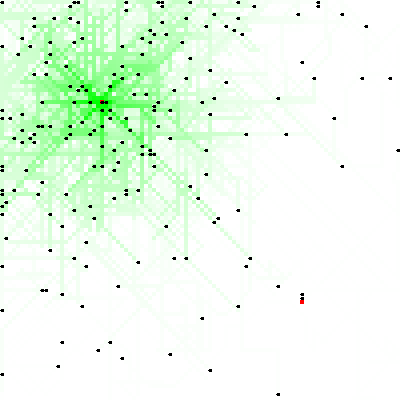
\includegraphics[width=0.3\textwidth]{ameisenmod1}}
		\fbox{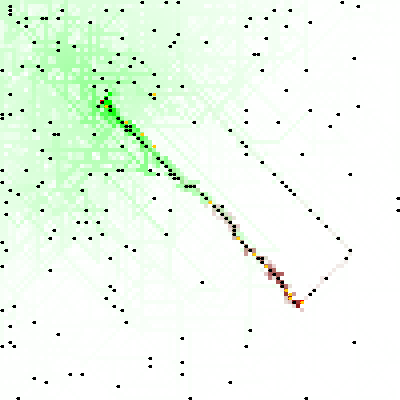
\includegraphics[width=0.3\textwidth]{ameisenmod2}}
		\fbox{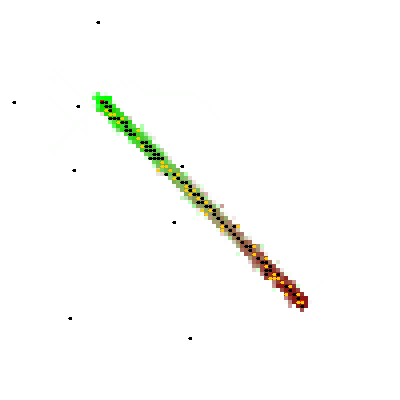
\includegraphics[width=0.3\textwidth]{ameisenmod3}}
	\end{center}
	\hspace{1in}\parbox{4in}{\caption[Bildung einer Ameisenstraße in der Simulation der Futtersuche von Ameisen]{Bildung einer Ameisenstraße in der Simulation der Futtersuche von Ameisen}}
	\label{acomodabb1}
\end{figure}
\subsubsection{Auswirkungen der Parameter auf die Ergebnisse der Simulation}
Die Strategie der Ameisen eine direkte, durch Pheromone markierte, Verbindung zwischen Ameisenbau und Futterquelle zu bilden wird durch den Parameter $\alpha$ gestört. Abbildung 6 zeigt den Einfluss des Parameters $\alpha$. Die zufallsgesteuerte Suche nach der Futterquelle ist zur Beginn der Simulation jedoch notwendig, da keine Pheromonmarkierungen vorhanden sind. Wird die Simulation der Futtersuche mit einer geringen Anzahl an modellierten Ameisen durchgeführt, dauert es länger bis die Futterquelle von einer Ameise gefunden wird. Bei einer hohen Anzahl an modellierten Ameisen steigt die Wahrscheinlichkeit, dass die modellierten Ameisen die Futterquelle finden. In der Simulation werden die meisten Futtereinheiten mit geringem Parameter $\alpha$ gesammelt. \newline
\begin{figure}[h]
	\begin{center}
		\fbox{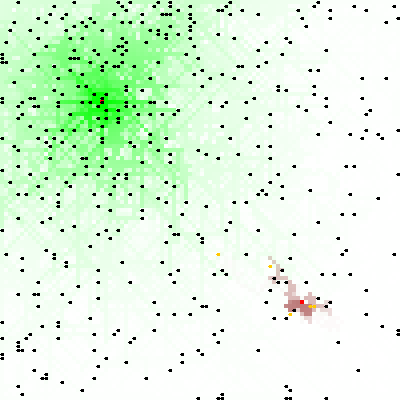
\includegraphics[width=0.3\textwidth]{ameisenmod4}}
		\fbox{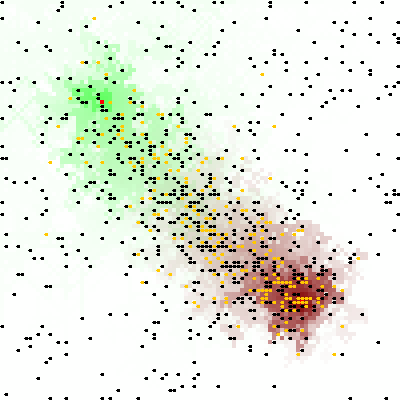
\includegraphics[width=0.3\textwidth]{ameisenmod5}}
		\fbox{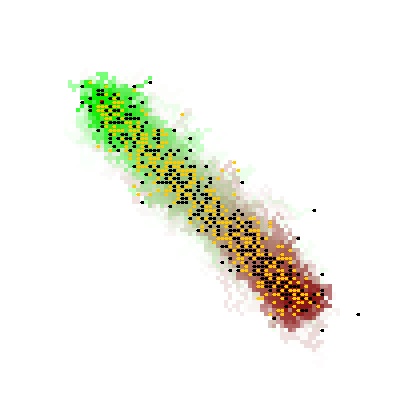
\includegraphics[width=0.3\textwidth]{ameisenmod6}}
	\end{center}
	\hspace{1in}\parbox{4in}{\caption[Einfluss des Parameters $\alpha$ in der Simulation der Futtersuche von Ameisen]{Einfluss des Parameters $\alpha$ in der Simulation der Futtersuche von Ameisen}}
	\label{acomodabb2}
\end{figure}
\subsection{Futtersuche von Bienen}
Wie in der Natur tanzen die modellierten Bienen, um anderen Bienen im Bienenstock die Richtung und Entfernung der Futterquelle zu zeigen. Da die Bienen im Bienenstock lediglich tanzende Bienen in ihrer direkten Umgebung sehen können, veranlasst eine tanzende Biene nur eine geringe Anzahl an Bienen dazu, ihr zur Futterquelle zu folgen. Kehren die rekrutierten Bienen erfolgreich von der Futterquelle zurück tanzen auch sie. Es entsteht eine Art Schneeballeffekt. Je mehr Bienen tanzen desto mehr Bienen bekommen die Information über die Richtung und Entfernung zur Futterquelle. Abbildung 7 zeigt den Abbau der Futterquelle in der Simulation.\newline
\begin{figure}[h]
	\begin{center}
		\fbox{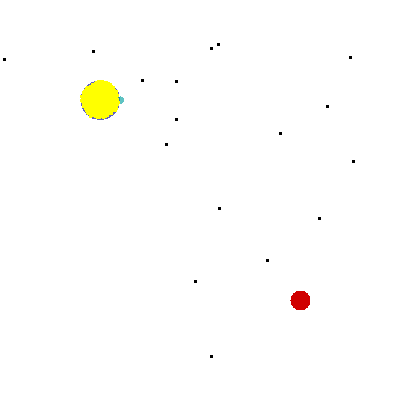
\includegraphics[width=0.3\textwidth]{bienenmod1}}
		\fbox{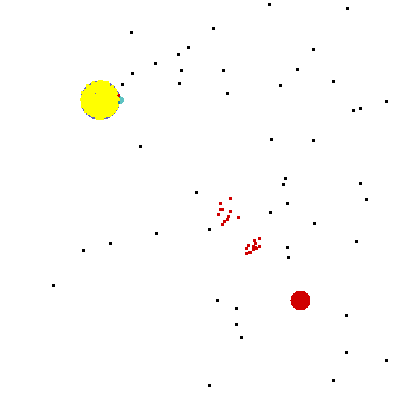
\includegraphics[width=0.3\textwidth]{bienenmod2}}
		\fbox{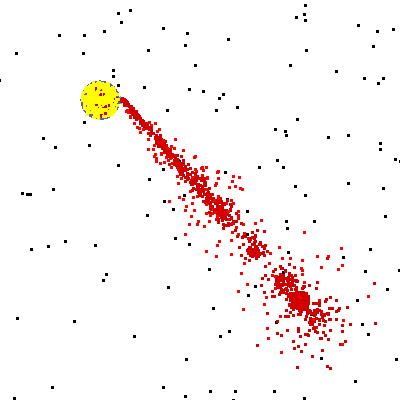
\includegraphics[width=0.3\textwidth]{bienenmod3}}
	\end{center}
	\hspace{1in}\parbox{4in}{\caption[Abbau der Futterquelle in der Simulation der Futtersuche von Bienen]{Abbau der Futterquelle in der Simulation der Futtersuche von Bienen}}
	\label{bcomodabb}
\end{figure}
\newpage
\section{Zusammenfassung}
Die Futtersuche von Ameisen und Bienen, anhand eines agentenbasierten Modells zu simulieren ist gelungen. Die Simulationen zeigen die typischen Strategien der Ameisen- und Bienenkolonien zum effizienten Abbau einer Futterquelle. Während die einzelnen modellierten Agenten nur über ein sehr beschränktes Repertoire an Fähigkeiten und Entscheidungsmöglichkeiten verfügen, entstehen bei einem Kollektiv an modellierten Agenten intelligente Lösungen auf Makroebene. Die modellierten Agenten besitzen dabei nur eine eingeschränkte Sicht auf das Gesamtsystem. Sie verfügen nur über die Informationen in ihrer unmittelbaren Umgebung. Wie in der Natur handeln die modellierten Agenten autonom. Sie entscheiden situationsbedingt welche der ihnen zur Verfügung stehenden Aktionen auszuführen ist.\newline \newline
Das in dieser Arbeit implementierte Modell der \acs{PSO} zum Finden des globalen Minimums der Rastrigin-Funktion liefert gute näherungsweise Lösungen. Das beste Resultat der im Rahmen dieser Arbeit durchgeführten Simulationen ist die näherungsweise Lösung $x = 0.0008121$ mit $f(x) = 0.00052893$, während sich das globale Minimum der Rastrigin-Funktion bei $x = 0$ mit $f(x)= 0$ befindet. 
\newpage
\begin{thebibliography}{sotief}
	\bibitem{1}A. Aulinger. Kollektive Intelligenz: Methoden, Erfahrungen und Perspektiven. Steinbeis-Edition. ISBN: 978-3941317151. Entstehungsjahr: 2009.	

	\bibitem{2}E. Bonabeau. Agent-based modeling: Methods and techniques for simulating human systems. National Academy of Sciences. 99 (suppl 3) 7280-7287. Entstehungsjahr: 2002.
	
	\bibitem{3}M. Dorigo, M. Birattari, T. Stützle. Ant Coloncy Optimization. Computational Intelligence Magazine, pp 28-39. Entstehungsjahr: 2004.
	
	\bibitem{4}J. Kennedy, R. Eberhart. A New Optimizer Using Particle Swarm Theory. MHS'95, Proceedings of the Sixith International Symposium. Entstehungsjahr: 1995.
	
	\bibitem{5}Y. Liu. Partikelschwarmoptimierung für diskrete Probleme. Technische Universität München. Entstehungsjahr: 2014.\newline\newline
	Weblink: http://\%3A\%2F\%2Fwwwmayr.informatik.tu-muenchen.de\%2Fkonferenzen\newline\%2FFerienakademie14\%2Fslides\_papers\%2Fpaper\_Yushan\_Liu.pdf\&usg=\newline AOvVaw0y3oo34w9QhrreOniL4ILk \newline Einsichtnahme: 14.01.2018
	
	\bibitem{6}C. Macal, M. North. Tutorial on agent-based modelling and simulation. Journal of Simulation 4, Nr. 1, pp 151-162. Entstehungsjahr: 2010.
	
	\bibitem{7}L. Pintscher. Schwarmintelligenz. Universität Karlsruhe. Entstehungsjahr: ohne Jahr.\newline\newline
	Weblink: http://lydiapintscher.de/uni/schwarmintelligenz.pdf \newline Einsichtnahme: 14.01.2018
	
	\bibitem{8}S. Railsback, S. Lytinen, S. Jackson. Agent-based Simulation Platforms: Review and Development Recommendations. SIMULATION. Vol 82, Issue 9. Entstehungsjahr: 2006.
	
	\bibitem{9}S. Russel, P. Norvig. Artificial Intelligence: A Modern Approach. Prentice Hall, Upper Saddle River. Entstehungsjahr: 2009.
	
	\bibitem{10} D. Teodorovi\'{c}, P. Lu\u{c}i\'{c}. Bee system: Modeling combinatorial optimization transportation engineering problems by swarm intelligence. Preprints of the TRISTAN IV Triennial Symposium on Transportation Analysis, pp 441-445. Entstehungsjahr: 2001.
	
	\bibitem{11}R. Wehner. Miniaturgehirne und kollektive Intelligenz. Zur Evolution biologischer Komplexität. Züricher Universitätszeitschriften 3. Entstehungsjahr: 2001. 
	
	\bibitem{12}W.M. Wheeler. The Ant Colony as an Organism. Journal of Morphology Volume 22, Issue 2, Seite 307-325. Entstehungsjahr: 1911.\newline\newline
	Weblink: http://www3.interscience.wiley.com/journal/109914213/abstract \newline Einsichtnahme: 04.01.2018
	
	\bibitem{13}Wikipedia. Rastrigin-Funktion. Wikipedia, Die freie Enzyklopädie. Bearbeitungsstand: 1. Sep 2016, 07:34 UTC. \newline\newline 
	Weblink:https://de.wikipedia.org/w/index.php?title=Rastrigin-Funktion\&oldid=177349710\newline
	Einsichtnahme: 02.03.2018
	
	\bibitem{14}M. Wooldridge, N. Jennings. Intelligent Agents: Theory and Practice. Knowledge Engineering Review 10, Nr. 2, pp 115-152. Entstehungsjahr: 1995.	
\end{thebibliography}
\newpage
\appendix
\appendixtoc
\newpage
\section{Anhang}
\subsection{Experimente \acs{PSO}}
\subsubsection{Globaler Vertrauenskoeffizient = 0.3, lokaler Vertrauenskoeffizient = 0.7}
\begin{itemize}
	\item 1000 Partikel, 100 Iterationen
	\begin{table}[h]
		\begin{tabular}{p{2.5cm}|p{11cm}}
			Simulation & beste Lösung (Position(x,y))\\ \hline\hline
			1 & 0.01262632028506161,-0.013384001669769718\\ \hline
			2 & 0.0019848665525268316,0.000528938028764081\\ \hline
			3 & 0.0008120558872288797,0.00047645837213217135\\ \hline
			4 & 0.001151650858115083,0.002847968150353708\\ \hline
		\end{tabular}
		\caption{Ergebnisse Simulation \acs{PSO}: 1000 Partikel, 100 Iterationen, Globaler Vertrauenskoeffizient = 0.3, lokaler Vertrauenskoeffizient = 0.7}
		\label{tabframework}
	\end{table}
	\item 100 Partikel, 100 Iterationen
	\begin{table}[h]
		\begin{tabular}{p{2.5cm}|p{11cm}}
			Simulation & beste Lösung (Position(x,y))\\ \hline\hline
			1 & 0.9772663170332931,-0.015964212524956722\\ \hline
			2 & -0.012299255721850477,-0.033490171619710574\\ \hline
			3 & -0.012308005422580148,0.9809504459943033\\ \hline
			4 & -0.050978886961883685,0.9850664961084877\\ \hline
		\end{tabular}
		\caption{Ergebnisse Simulation \acs{PSO}: 100 Partikel, 100 Iterationen, Globaler Vertrauenskoeffizient = 0.3, lokaler Vertrauenskoeffizient = 0.7}
		\label{tabframework}
	\end{table}
\end{itemize}
\newpage
\subsubsection{Globaler Vertrauenskoeffizient = 0.5, lokaler Vertrauenskoeffizient = 0.5}
\begin{itemize}
	\item 1000 Partikel, 100 Iterationen
	\begin{table}[h]
		\begin{tabular}{p{2.5cm}|p{11cm}}
			Simulation & beste Lösung (Position(x,y))\\ \hline\hline
			1 & 0.01262632028506161,-0.013384001669769718\\ \hline
			2 & 0.0019848665525268316,0.000528938028764081\\ \hline
			3 & 0.0008120558872288797,0.00047645837213217135\\ \hline
			4 & 0.001151650858115083,0.002847968150353708\\ \hline
		\end{tabular}
		\caption{Ergebnisse Simulation \acs{PSO}: 1000 Partikel, 100 Iterationen, Globaler Vertrauenskoeffizient = 0.5, lokaler Vertrauenskoeffizient = 0.5}
		\label{tabframework}
	\end{table}
	\item 100 Partikel, 100 Iterationen
	\begin{table}[h]
		\begin{tabular}{p{2.5cm}|p{11cm}}
			Simulation & beste Lösung (Position(x,y))\\ \hline\hline
			1 & -0.020958980636341273,-0.01571132254960461\\ \hline
			2 & -0.032716891537396986,-0.008106273053844149\\ \hline
			3 & -0.01916372314789072,-0.9962361142871572\\ \hline
			4 & 0.005898689367579202,-0.025737966396528478\\ \hline
		\end{tabular}
		\caption{Ergebnisse Simulation \acs{PSO}: 100 Partikel, 100 Iterationen, Globaler Vertrauenskoeffizient = 0.5, lokaler Vertrauenskoeffizient = 0.5}
		\label{tabframework}
	\end{table}
\end{itemize}
\newpage
\subsubsection{Globaler Vertrauenskoeffizient = 0.7, lokaler Vertrauenskoeffizient = 0.3}
\begin{itemize}
	\item 1000 Partikel, 100 Iterationen
	\begin{table}[h]
		\begin{tabular}{p{2.5cm}|p{11cm}}
			Simulation & beste Lösung (Position(x,y))\\ \hline\hline
			1 & 0.01262632028506161,-0.013384001669769718\\ \hline
			2 & 0.0019848665525268316,0.000528938028764081\\ \hline
			3 & 0.0008120558872288797,0.00047645837213217135\\ \hline
			4 & 0.001151650858115083,0.002847968150353708\\ \hline
		\end{tabular}
		\caption{Ergebnisse Simulation \acs{PSO}: 1000 Partikel, 100 Iterationen, Globaler Vertrauenskoeffizient = 0.7, lokaler Vertrauenskoeffizient = 0.3}
		\label{tabframework}
	\end{table}
	\item 100 Partikel, 100 Iterationen
	\begin{table}[h]
		\begin{tabular}{p{2.5cm}|p{11cm}}
			Simulation & beste Lösung (Position(x,y))\\ \hline\hline
			1 & 0.9772663170332931,-0.015964212524956722\\ \hline
			2 & -0.012299255721850477,-0.033490171619710574\\ \hline
			3 & -0.012308005422580148,0.9809504459943033\\ \hline
			4 & -0.050978886961883685,0.9850664961084877\\ \hline
		\end{tabular}
		\caption{Ergebnisse Simulation \acs{PSO}: 100 Partikel, 100 Iterationen, Globaler Vertrauenskoeffizient = 0.7, lokaler Vertrauenskoeffizient = 0.3}
		\label{tabframework}
	\end{table}
\end{itemize}
\newpage

\subsection{Experimente Futtersuche von Ameisen}
\subsubsection{$\alpha$ = 0.3, $\beta$ = 0.7}
\begin{itemize}
	\item 1000 Ameisen, 5000 Iterationen
	\begin{table}[h]
		\begin{tabular}{p{2.5cm}|p{11cm}}
			Simulation & gesammelte Futtereinheiten\\ \hline\hline
			1 & 27190\\ \hline
			2 & 25918\\ \hline
			3 & 25535\\ \hline
			4 & 25841\\ \hline
		\end{tabular}
		\caption{Ergebnisse Simulation der Futtersuche von Ameisen: 1000 Ameisen, 5000 Iterationen, $\alpha$ = 0.3, $\beta$ = 0.7}
		\label{tabframework}
	\end{table}
	\item 100 Ameisen, 5000 Iterationen
	\begin{table}[h]
		\begin{tabular}{p{2.5cm}|p{11cm}}
			Simulation & gesammelte Futtereinheiten\\ \hline\hline
			1 & 2453\\ \hline
			2 & 2465\\ \hline
			3 & 2528\\ \hline
			4 & 2529\\ \hline
		\end{tabular}
		\caption{Ergebnisse Simulation der Futtersuche von Ameisen: 100 Ameisen, 5000 Iterationen, $\alpha$ = 0.3, $\beta$ = 0.7}
		\label{tabframework}
	\end{table}
\end{itemize}
\newpage
\subsubsection{$\alpha$ = 0.5, $\beta$ = 0.5}
\begin{itemize}
	\item 1000 Ameisen, 5000 Iterationen
	\begin{table}[h]
		\begin{tabular}{p{2.5cm}|p{11cm}}
			Simulation & gesammelte Futtereinheiten\\ \hline\hline
			1 & 16106\\ \hline
			2 & 16758\\ \hline
			3 & 16504\\ \hline
			4 & 15972\\ \hline
		\end{tabular}
		\caption{Ergebnisse Simulation der Futtersuche von Ameisen: 1000 Ameisen, 5000 Iterationen, $\alpha$ = 0.5, $\beta$ = 0.5}
		\label{tabframework}
	\end{table}
	\item 100 Ameisen, 5000 Iterationen
	\begin{table}[h]
		\begin{tabular}{p{2.5cm}|p{11cm}}
			Simulation & gesammelte Futtereinheiten\\ \hline\hline
			1 & 1110\\ \hline
			2 & 1428\\ \hline
			3 & 996\\ \hline
			4 & 1277\\ \hline
		\end{tabular}
		\caption{Ergebnisse Simulation der Futtersuche von Ameisen: 100 Ameisen, 5000 Iterationen, $\alpha$ = 0.5, $\beta$ = 0.5}
		\label{tabframework}
	\end{table}
\end{itemize}
\newpage
\subsubsection{$\alpha$ = 0.7, $\beta$ = 0.3}
\begin{itemize}
	\item 1000 Partikel, 100 Iterationen
	\begin{table}[h]
		\begin{tabular}{p{2.5cm}|p{11cm}}
			Simulation & beste Lösung (Position(x,y))\\ \hline\hline
			1 & 9951\\ \hline
			2 & 9628\\ \hline
			3 & 9428\\ \hline
			4 & 8923\\ \hline
		\end{tabular}
		\caption{Ergebnisse Simulation der Futtersuche von Ameisen: 1000 Ameisen, 5000 Iterationen, $\alpha$ = 0.7, $\beta$ = 0.3}
		\label{tabframework}
	\end{table}
	\item 100 Partikel, 100 Iterationen
	\begin{table}[h]
		\begin{tabular}{p{2.5cm}|p{11cm}}
			Simulation & beste Lösung (Position(x,y))\\ \hline\hline
			1 & 709\\ \hline
			2 & 595\\ \hline
			3 & 812\\ \hline
			4 & 772\\ \hline
		\end{tabular}
		\caption{Ergebnisse Simulation der Futtersuche von Ameisen: 100 Ameisen, 5000 Iterationen, $\alpha$ = 0.7, $\beta$ = 0.3}
		\label{tabframework}
	\end{table}
\end{itemize}
\newpage

\subsection{Experimente Futtersuche von Bienen}
\begin{itemize}
	\item 2000 Bienen, 5000 Iterationen
	\begin{table}[h]
		\begin{tabular}{p{2.5cm}|p{11cm}}
			Simulation & gesammelte Futtereinheiten\\ \hline\hline
			1 & 1822\\ \hline
			2 & 2152\\ \hline
			3 & 2395\\ \hline
			4 & 1841\\ \hline
		\end{tabular}
		\caption{Ergebnisse Simulation der Futtersuche von Bienen: 2000 Bienen, 5000 Iterationen}
		\label{tabframework}
	\end{table}
	\item 1000 Bienen, 5000 Iterationen
	\begin{table}[h]
		\begin{tabular}{p{2.5cm}|p{11cm}}
			Simulation & gesammelte Futtereinheiten\\ \hline\hline
			1 & 805\\ \hline
			2 & 1146\\ \hline
			3 & 830\\ \hline
			4 & 996\\ \hline
		\end{tabular}
		\caption{Ergebnisse Simulation der Futtersuche von Bienen: 1000 Bienen, 5000 Iterationen}
		\label{tabframework}
	\end{table}
	\item 100 Ameisen, 5000 Iterationen
	\begin{table}[h]
		\begin{tabular}{p{2.5cm}|p{11cm}}
			Simulation & gesammelte Futtereinheiten\\ \hline\hline
			1 & 11\\ \hline
			2 & 4\\ \hline
			3 & 40\\ \hline
			4 & 69\\ \hline
		\end{tabular}
		\caption{Ergebnisse Simulation der Futtersuche von Bienen: 100 Bienen, 5000 Iterationen}
		\label{tabframework}
	\end{table}
\end{itemize}
\end{document}


